\documentclass[12pt, a4paper, oneside]{ctexart}
\usepackage{amsmath, amsthm, amssymb, bm, color, graphicx, geometry, mathrsfs,extarrows, braket, booktabs, array, xcolor, fontspec, appendix, float, subfigure, wrapfig, enumitem, titlesec, tabularx}
\usepackage[colorlinks,linkcolor=black,anchorcolor=blue,citecolor=blue,urlcolor=blue,menucolor=black]{hyperref}

%%%% 设置中文字体 %%%%
% fc-list -f "%{family}\n" :lang=zh >d:zhfont.txt 命令查看已有字体
\setCJKmainfont[
    BoldFont=方正黑体_GBK,  % 黑体
    ItalicFont=方正楷体_GBK,  % 楷体
    BoldItalicFont=方正粗楷简体,  % 粗楷体
    Mapping = fullwidth-stop  % 将中文句号“.”全部转化为英文句号“.”,
]{方正书宋简体}  % !!! 注意在Windows中运行请改为“方正书宋简体.ttf” !!!
%%%% 设置英文字体 %%%%
\setmainfont{Minion Pro}
\setsansfont{Calibri}
\setmonofont{Consolas}

%%%% 设置代码块 %%%%
% 在vscode中使用minted需要先配置python解释器, Ctrl+Shift+P, 输入Python: Select Interpreter选择安装了Pygments的Python版本. 再在setting.json中xelatex和pdflatex的参数中加入 "--shell-escape", 即可
% TeXworks中配置方法参考: https://blog.csdn.net/RobertChenGuangzhi/article/details/108140093
\usepackage{minted}
\renewcommand{\theFancyVerbLine}{
    \sffamily\textcolor[rgb]{0.5,0.5,0.5}{\scriptsize\arabic{FancyVerbLine}}} % 修改代码前序号大小
% 加入不同语言的代码块
\newmintinline{cpp}{fontsize=\small, linenos, breaklines, frame=lines}
\newminted{cpp}{fontsize=\small, baselinestretch=1, linenos, breaklines, frame=lines}
\newmintedfile{cpp}{fontsize=\small, baselinestretch=1, linenos, breaklines, frame=lines}
\newmintinline{matlab}{fontsize=\small, linenos, breaklines, frame=lines}
\newminted{matlab}{fontsize=\small, baselinestretch=1, mathescape, linenos, breaklines, frame=lines}
\newmintedfile{matlab}{fontsize=\small, baselinestretch=1, linenos, breaklines, frame=lines}
\newmintinline{python}{fontsize=\small, linenos, breaklines, frame=lines, python3}  % 使用\pythoninline{代码}
\newminted{python}{fontsize=\small, baselinestretch=1, linenos, breaklines, frame=lines, python3}  % 使用\begin{pythoncode}代码\end{pythoncode}
\newmintedfile{python}{fontsize=\small, baselinestretch=1, linenos, breaklines, frame=lines, python3}  % 使用\pythonfile{代码地址}
\newcommand{\mypythonfile}[1]{
  \vspace{-2ex}
  \pythonfile{#1}
  \vspace{-2ex}
}

%%%% 设置行间距与页边距 %%%%
\linespread{1.2}
\geometry{left=2.5cm, right=2.5cm, top=2.5cm, bottom=2.5cm}
% \geometry{left=1.84cm,right=1.84cm,top=2.18cm,bottom=2.18cm}  % 更小的页边距

%%%% 定理类环境的定义 %%%%
\newtheorem{example}{例}            % 整体编号
\newtheorem{theorem}{定理}[section] % 定理按section编号
\newtheorem{definition}{定义}
\newtheorem{axiom}{公理}
\newtheorem{property}{性质}
\newtheorem{proposition}{命题}
\newtheorem{lemma}{引理}
\newtheorem{corollary}{推论}
\newtheorem{condition}{条件}
\newtheorem{conclusion}{结论}
\newtheorem{assumption}{假设}
\numberwithin{equation}{section}  % 公式按section编号 (公式右端的小括号)
\newtheorem{algorithm}{算法}

%%%% 自定义环境 %%%%
\newsavebox{\nameinfo}
\newenvironment{myTitle}[1]{
    \begin{center}
    {\zihao{-2}\bf #1\\}
    \zihao{-4}\it
}{\end{center}}  % \begin{myTitle}{标题内容}作者信息\end{myTitle}
\newcounter{problem}[subsection]  % 问题序号计数器
\newenvironment{problem}[1][]{\stepcounter{problem}\par\noindent\textbf{题目\thesubsection.\arabic{problem}. #1}}{\smallskip\par}
\newenvironment{solution}[1][]{\par\noindent\textbf{#1解答. }}{\smallskip\par}  % 可带一个参数表示题号\begin{solution}{题号}
\newenvironment{note}{\par\noindent\textbf{注记. }}{\smallskip\par}
\newenvironment{remark}{\begin{enumerate}[label=\textbf{注\arabic*.}]}{\end{enumerate}}
\BeforeBeginEnvironment{minted}{\vspace{-0.5cm}}  % 缩小minted环境距上文间距
\AfterEndEnvironment{minted}{\vspace{-0.2cm}}  % 缩小minted环境距下文间距

%%%% 自定义段落开头序号,间距 (titlesec) %%%%
% 中文序号:\zhnum{section}, 阿拉伯序号:\arabic
\titleformat{\section}{\Large\bfseries}{\arabic{section}}{1em}{}[]
\titlespacing{\section}{0pt}{1.2ex plus .0ex minus .0ex}{.6ex plus .0ex}
\titlespacing{\subsection}{0pt}{1.2ex plus .0ex minus .0ex}{.6ex plus .0ex}
\titlespacing{\subsubsection}{0pt}{1.2ex plus .0ex minus .0ex}{.6ex plus .0ex}

%%%% 图片相对路径 %%%%
\graphicspath{{figures/}} % 当前目录下的figures文件夹, {../figures/}则是父目录的figures文件夹
\setlength{\abovecaptionskip}{-0.1cm}  % 缩紧图片标题与图片之间的距离
\setlength{\belowcaptionskip}{0pt} 

%%%% 缩小item,enumerate,description两行间间距 %%%%
\setenumerate[1]{itemsep=0pt,partopsep=0pt,parsep=\parskip,topsep=5pt}
\setitemize[1]{itemsep=0pt,partopsep=0pt,parsep=\parskip,topsep=5pt}
\setdescription{itemsep=0pt,partopsep=0pt,parsep=\parskip,topsep=5pt}

%%%% 自定义公式 %%%%
\everymath{\displaystyle} % 默认全部行间公式, 想要变回行内公式使用\textstyle
\DeclareMathOperator*\uplim{\overline{lim}}     % 定义上极限 \uplim_{}
\DeclareMathOperator*\lowlim{\underline{lim}}   % 定义下极限 \lowlim_{}
\DeclareMathOperator*{\argmax}{arg\,max}  % 定义取最大值的参数 \argmax_{}
\DeclareMathOperator*{\argmin}{arg\,min}  % 定义取最小值的参数 \argmin_{}
\let\leq=\leqslant % 简写小于等于\leq (将全部leq变为leqslant)
\let\geq=\geqslant % 简写大于等于\geq (将全部geq变为geqslant)
\DeclareRobustCommand{\rchi}{{\mathpalette\irchi\relax}}
\newcommand{\irchi}[2]{\raisebox{\depth}{$#1\chi$}} % 使用\rchi将\chi居中

%%%% 一些宏定义 %%%%
\def\bd{\boldsymbol}        % 加粗(向量) boldsymbol
\def\disp{\displaystyle}    % 使用行间公式 displaystyle(默认)
\def\tsty{\textstyle}       % 使用行内公式 textstyle
\def\sign{\text{sign}}      % sign function
\def\wtd{\widetilde}        % 宽波浪线 widetilde
\def\R{\mathbb{R}}          % Real number
\def\N{\mathbb{N}}          % Natural number
\def\Z{\mathbb{Z}}          % Integer number
\def\Q{\mathbb{Q}}          % Rational number
\def\C{\mathbb{C}}          % Complex number
\def\K{\mathbb{K}}          % Number Field
\def\P{\mathbb{P}}          % Polynomial
\def\E{\mathbb{E}}          % Exception
\def\d{\mathrm{d}}          % differential operator
\def\e{\mathrm{e}}          % Euler's number
\def\i{\mathrm{i}}          % imaginary number
\def\re{\mathrm{Re}}        % Real part
\def\im{\mathrm{Im}}        % Imaginary part
\def\res{\mathrm{Res}}      % Residue
\def\ker{\mathrm{Ker}}      % Kernel
\def\vspan{\mathrm{vspan}}  % Span  \span与latex内核代码冲突改为\vspan
\def\L{\mathcal{L}}         % Loss function
\def\O{\mathcal{O}}         % big O notation
\def\wdh{\widehat}          % 宽帽子 widehat
\def\ol{\overline}          % 上横线 overline
\def\ul{\underline}         % 下横线 underline
\def\add{\vspace{1ex}}      % 增加行间距
\def\del{\vspace{-1.5ex}}   % 减少行间距

%%%% 正文开始 %%%%
\begin{document}

% 单人封面
\begin{titlepage}
\begin{figure}[htbp]
  \centering
  
\includegraphics[width=0.8\linewidth]{红色校徽文字.png}
\end{figure}
\centering\bfseries\zihao{1} 文本分析与图像处理作业\\[5ex]
{
  \zihao{3}
  \begin{center}
    姓名:吴天阳\\
    学号:4124136039\\
  \end{center}
}
{
  \vfill
  \begin{center}
  \zihao{3} 
  西安交通大学\quad 人工智能学院\\[2ex]
  \today % 日期置底
  \end{center}
}
\end{titlepage}
\clearpage
\tableofcontents % 创建目录页,使用目录需要编译两次, 并且不能删去编译产生的临时文件!!!
\clearpage

\section{Chapter1}
\subsection{自然语言处理与文本挖掘基础}
\begin{problem}
在网络上用(Baidu, Google, Bing等)搜索关键词,判断搜索结果是否合理?
\end{problem}
\begin{solution}
比较合理,只需要手动分辨前面的广告内容
\end{solution}
\begin{problem}
了解自然语言处理编程工具(见前面PPT)
\end{problem}
\begin{solution}
常用的 Python 自然语言处理工具包括:
\begin{itemize}
  \item \textbf{NLTK (Natural Language Toolkit)}:一个功能全面的 NLP 工具包,支持分词、词性标注、命名实体识别、句法分析等基础操作,适合教学与研究用途。
  \item \textbf{spaCy}:注重工业级性能,适合大规模文本处理,内置高效的语言模型,可进行依存句法分析、词性标注及实体识别等任务。
  \item \textbf{TextBlob}:基于 NLTK 和 Pattern 构建,提供简单的 API,适用于快速原型开发和情感分析。
  \item \textbf{Transformers (Hugging Face)}:现代 NLP 核心工具库,提供多种预训练语言模型(如 BERT、GPT、T5 等),广泛应用于文本分类、问答、摘要生成等高级任务。
  \item \textbf{Gensim}:专注于词向量建模与主题建模,支持 Word2Vec、Doc2Vec 及 LDA 等模型,适合语义分析和文本聚类应用。
\end{itemize}
\end{solution}
\begin{problem}
了解Baidu, 谷歌等公司的NLP研究组/API工具:
\url{https://nlp.baidu.com/homepage/index},
\url{Google Natural Language API - Powerful Text Analysis}
\end{problem}
\begin{solution}
\textbf{百度自然语言处理平台(Baidu NLP)}
百度 NLP 平台是百度基于深度学习技术构建的中文自然语言处理服务系统,
面向开发者提供丰富的文本分析能力。该平台支持多种功能模块,包括:
\begin{itemize}
  \item 文本分类、情感分析、关键词提取、摘要生成;
  \item 分词、词性标注、依存句法分析、命名实体识别;
  \item 对话理解、意图识别及知识图谱构建支持。
\end{itemize}
百度 NLP 平台集成了预训练模型与大规模知识库,广泛应用于智能客服、舆情分析、智能写作等中文处理场景,并通过 RESTful API 接口提供在线调用能力。

\textbf{Google Natural Language API}
谷歌自然语言API是 Google Cloud 提供的文本智能分析服务,
支持多语言处理,面向全球开发者开放。主要功能包括:
\begin{itemize}
  \item 实体识别与分类、情感分析、句法分析;
  \item 文档分类、内容语言检测;
  \item 与 Google Cloud Translation、Speech 等服务无缝集成。
\end{itemize}
Google Natural Language API 支持 REST 和 gRPC 接口,基于 Google 多年积累的大模型能力,
在文本理解、信息抽取等方面具有强大的性能,适合构建跨语言、跨领域的智能文本系统。
\end{solution}

\subsection{Introduction 2023 图像处理概述}
\begin{problem}
了解和学习python/pytorch/matlab的图像软件包,包括读取、显示下载的图像、并转存为不同格式的图像,
查看一下不同格式下图像文件的大小.
\end{problem}
\begin{solution}
在Pytorch中也是使用PIL来读取图片,因此安装所需的包为\texttt{pip install pillow matplotlib},
代码如下:
\mypythonfile{./coding/prob1.2.1\(1\).py}

\clearpage
输出结果为(不同的图像大小比较):
\begin{pythoncode}
format       size(KB)
----------------------
JPG(ORG)        47.34
PNG            114.29
JPEG            25.19
BMP            342.05
TIFF           341.80
WEBP             8.08
PDF             26.06
\end{pythoncode}
效果图如下:
\begin{figure}[H]
  \centering
  \subfigure[原图JPG]{
\includegraphics[width=0.32\textwidth]{./coding/img.jpg}}
  \subfigure[PNG]{
\includegraphics[width=0.32\textwidth]{./coding/1.2.1_results/img.png}}
  \subfigure[JPEG]{
\includegraphics[width=0.32\textwidth]{./coding/1.2.1_results/img.jpeg}}
  \subfigure[BMP]{
\includegraphics[width=0.32\textwidth]{./coding/1.2.1_results/img.bmp}}
  % \subfigure[TIFF]{
\includegraphics[width=0.32\textwidth]{./coding/1.2.1_results/img.tiff}}
  % \subfigure[WEBP]{
\includegraphics[width=0.32\textwidth]{./coding/1.2.1_results/img.webp}}
  \subfigure[PDF]{
\includegraphics[width=0.32\textwidth]{./coding/1.2.1_results/img.pdf}}
  \setlength{\abovecaptionskip}{0ex}  % 如果使用了minted会增大图像与标题间距需要进行缩小
  \caption{不同的图像保存结果效果对比(LaTeX不支持\texttt{tiff}和\texttt{webp}文件)}
\end{figure}
\end{solution}
\begin{problem}
继续2,显示图像矩阵的内容、显示图像块、理解图像表示中所讲解的内容。
\end{problem}
\begin{solution}
通过对\texttt{np.ndarray}求切片即可获得图像的每个通道上像素的信息,这里我们取出图像中的正中心40x40的像素显示出来,
并显示不同通道上的图像,代码如下
\mypythonfile{./coding/prob1.2.1\(2\).py}
代码输出如下:
\begin{pythoncode}
Image shape (Height x Width x Channels): (342, 341, 3)
Top-left 5x5 pixel values of the red channel:
[[255 255 255 255 255]
 [255 255 255 255 255]
 [255 255 255 255 255]
 [255 255 255 255 255]
 [255 255 255 255 255]]
\end{pythoncode}
\clearpage
效果图如下
\begin{figure}[H]
  \centering
  \subfigure[图像中心40x40区块]{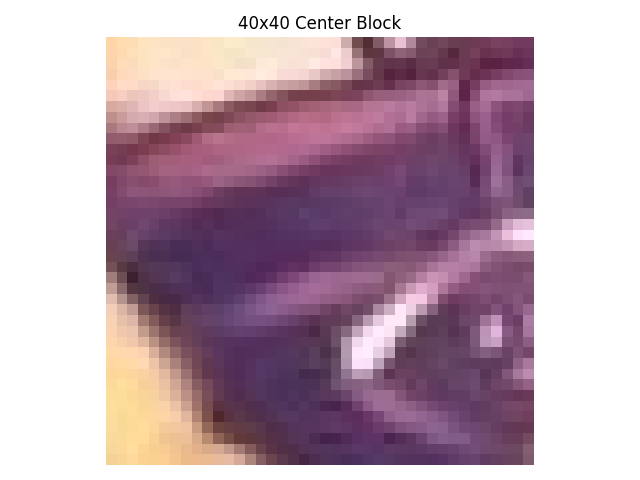
\includegraphics[width=0.3\textwidth]{./coding/1.2.1_results/40x40_center_block.png}}
  \subfigure[不同的通道上的图像]{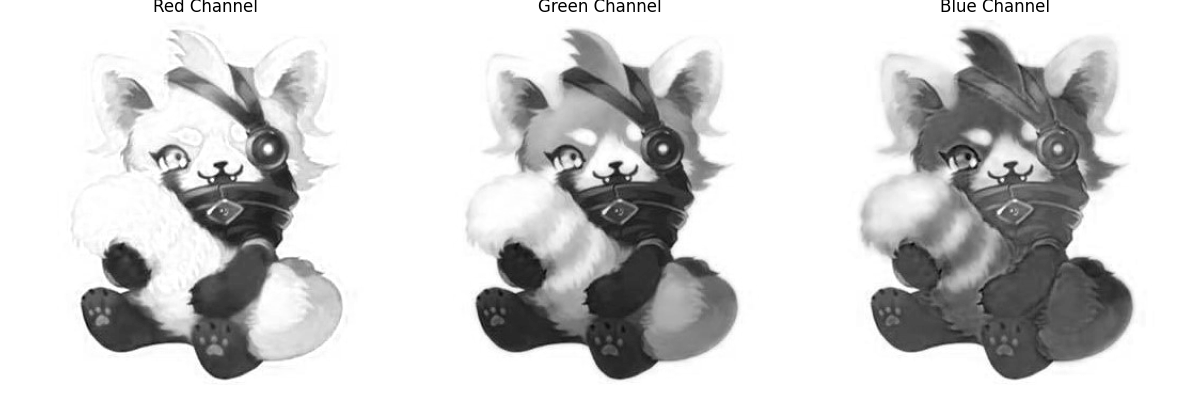
\includegraphics[width=0.69\textwidth]{./coding/1.2.1_results/show_diff_channels.png}}
  \setlength{\abovecaptionskip}{0ex}  % 如果使用了minted会增大图像与标题间距需要进行缩小
  \caption{效果图}
\end{figure}
\end{solution}

\section{Chapter2}
\subsection{分词、句法、文本表示}
\begin{problem}
作业:尝试汉语分词工具;学习并运行word2vec的代码:\url{https://github.com/fxsjy/jieba}, \url{https://github.com/loretoparisi/word2vec}
\end{problem}
\begin{solution}
安装所需包\texttt{pip install jieba gensim},完成上述任务。

\noindent\textbf{使用汉语分词工具}:使用\texttt{jieba}对《静夜思》进行分词,并给出高频词:
\mypythonfile{./coding/prob2.1.1\(1\).py}
运行结果:
\begin{pythoncode}
Building prefix dict from the default dictionary ...
Loading model from cache /tmp/jieba.cache
Loading model cost 0.433 seconds.
Prefix dict has been built successfully.
分词结果: ['床前', '明月光', ',', '疑是', '地上', '霜', '。', '\n', '举头', '望明月', ',', '低头', '思', '故乡', '。']
高频词: [(',', 2), ('。', 2), ('床前', 1)]
\end{pythoncode}

\noindent\textbf{学习并运行 Word2Vec}:使用\texttt{gensim}训练自己的词向量,并找出和“国王”相似的词语
\mypythonfile{./coding/prob2.1.1\(2\).py}
运行结果:
\begin{pythoncode}
[('王子', 0.044917721301317215), ('女人', -0.010146037675440311), ('是', -0.014475268311798573), ('儿子', -0.04407211393117905), ('男人', -0.12279318273067474), ('王后', -0.15515565872192383), ('的', -0.17424817383289337), ('女儿', -0.20600517094135284), ('公主', -0.2091004103422165)]
\end{pythoncode}
\end{solution}

\subsection{Geometry \& histogram}
\begin{problem}
拍摄或选取一幅低光条件下拍摄的相片,通过Python程序实现直方图均衡化、规定化,并观察效果。
\end{problem}
\begin{solution}
使用\texttt{skimage, opencv-python}包进行直方图处理,使用\texttt{pip}安装\texttt{pip install scikit-image PyWavelets opencv-python},代码如下
\mypythonfile{./coding/prob2.2.1.py}
效果图如下
\begin{figure}[htbp]
  \centering
  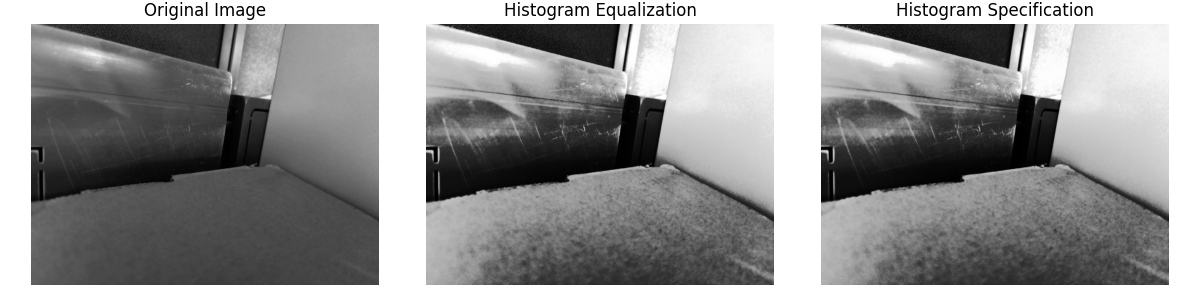
\includegraphics[width=\linewidth]{./coding/2.2.1_results/processed_results.png}
  \caption{直方图处理后对比效果图}
\end{figure}
\begin{figure}[htbp]
  \centering
  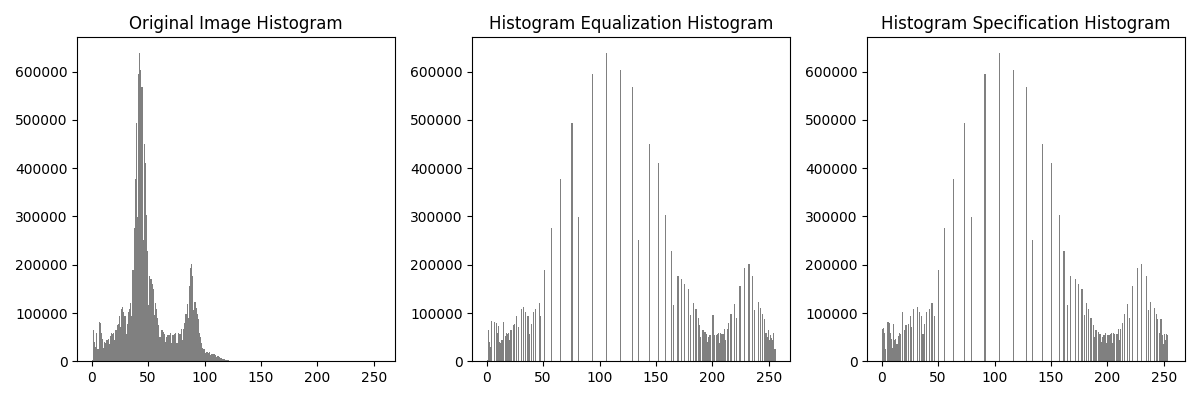
\includegraphics[width=\linewidth]{./coding/2.2.1_results/histogram_results.png}
  \caption{处理后的直方图}
\end{figure}
\end{solution}

\begin{problem}
尝试图像处理软件Photoshop的图像调节软件
Image -> Adjustments -> Brightness / contrast、Levels、Curves、Exposure
\end{problem}
\begin{solution}
使用PS处理后的效果如下
\begin{figure}[H]
  \centering
  \subfigure[原图]{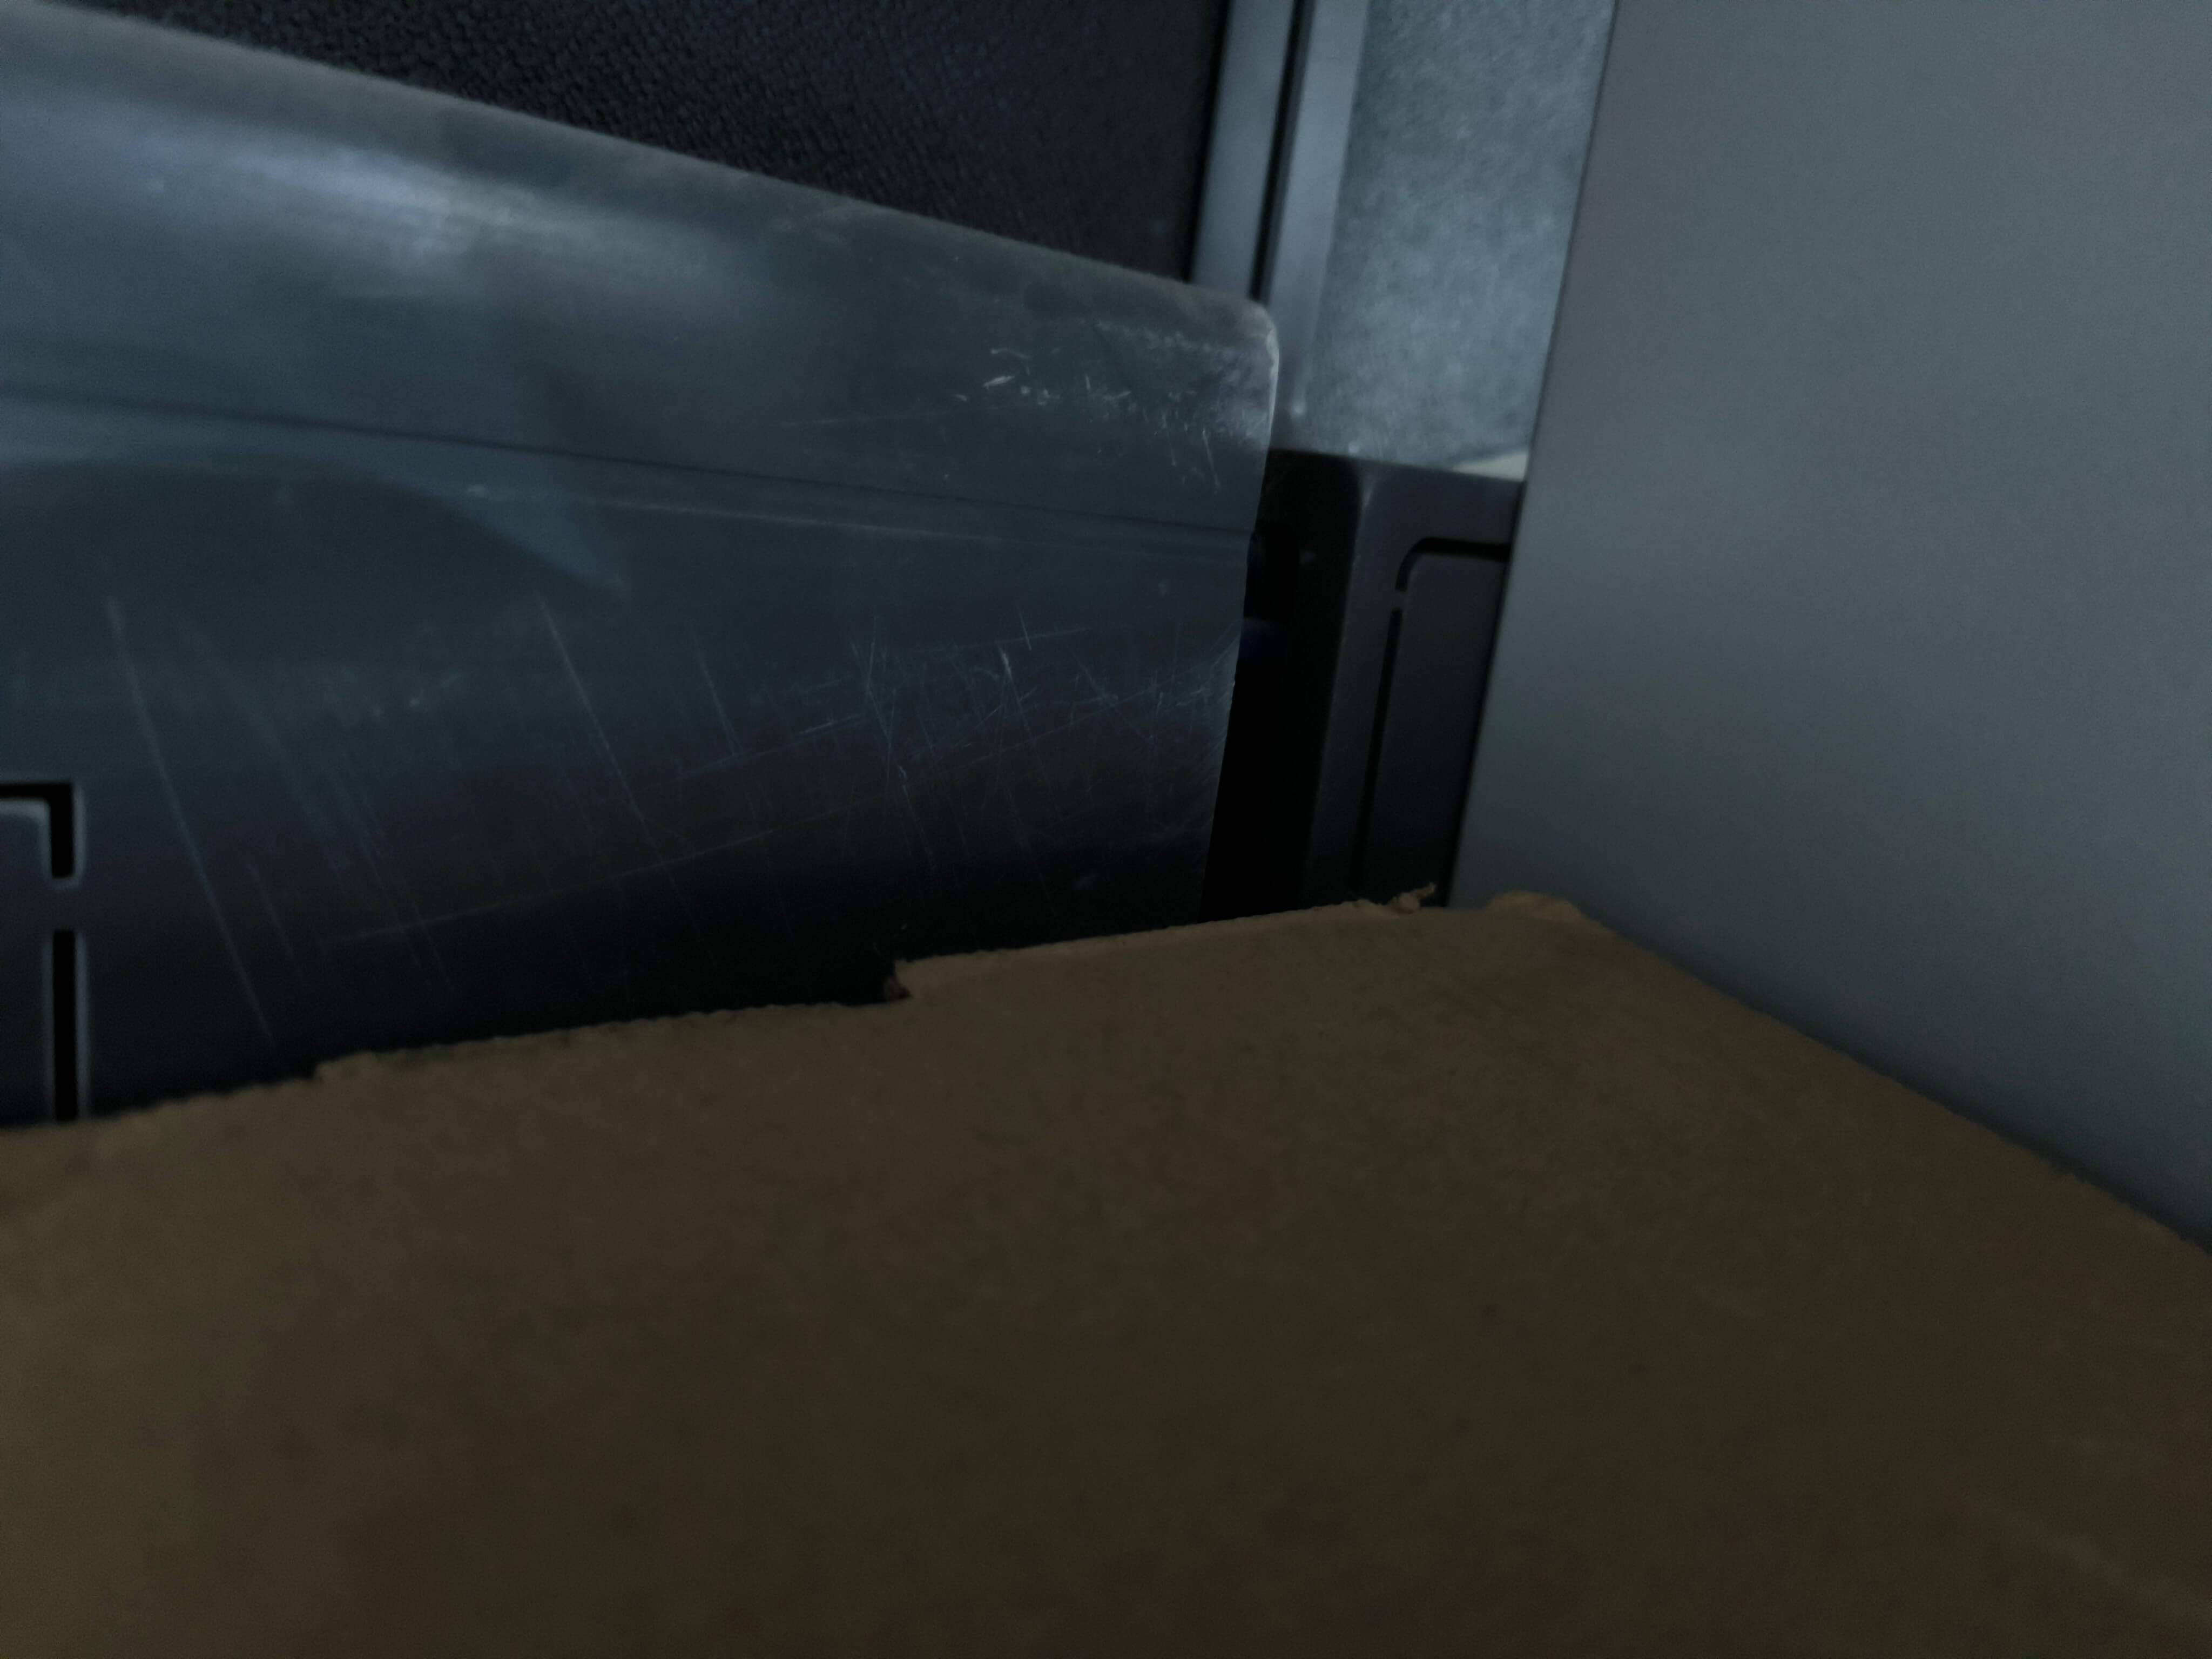
\includegraphics[width=0.32\textwidth]{./coding/low_light.jpg}}
  \subfigure[brightness/contrast]{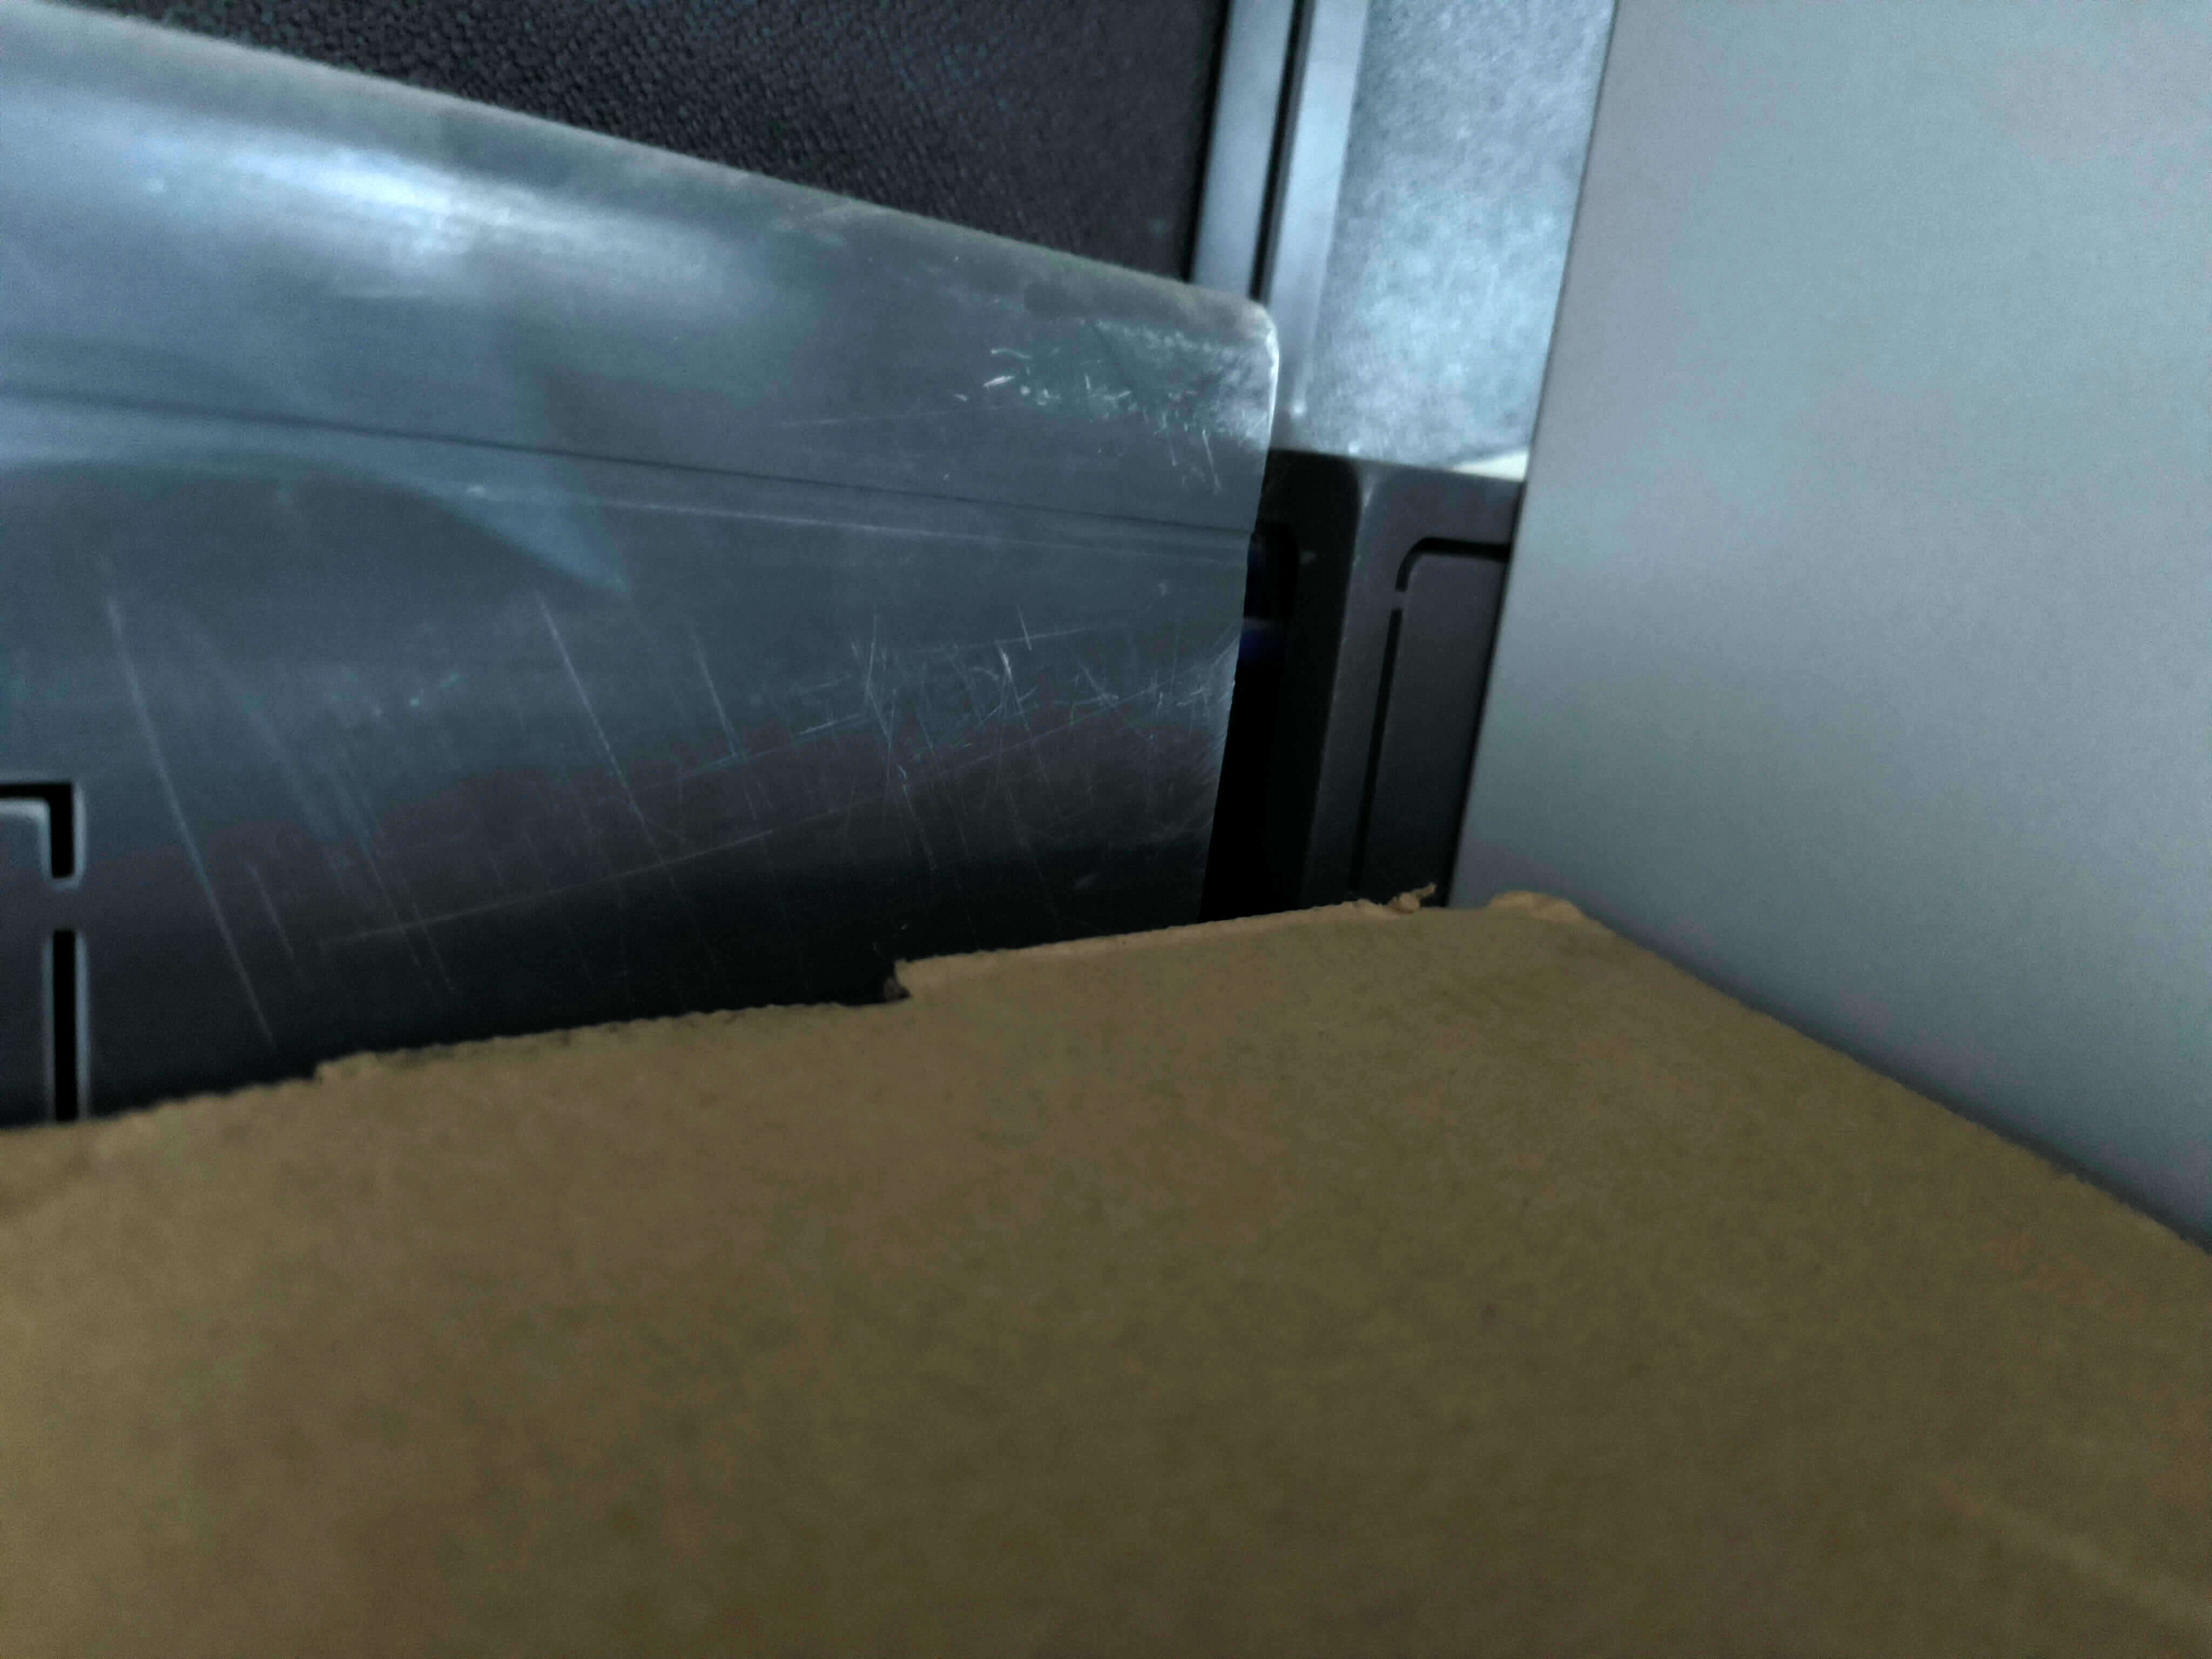
\includegraphics[width=0.32\textwidth]{./coding/2.2.1_results/low_light_brightness_contrast.jpg}}
  \subfigure[levels]{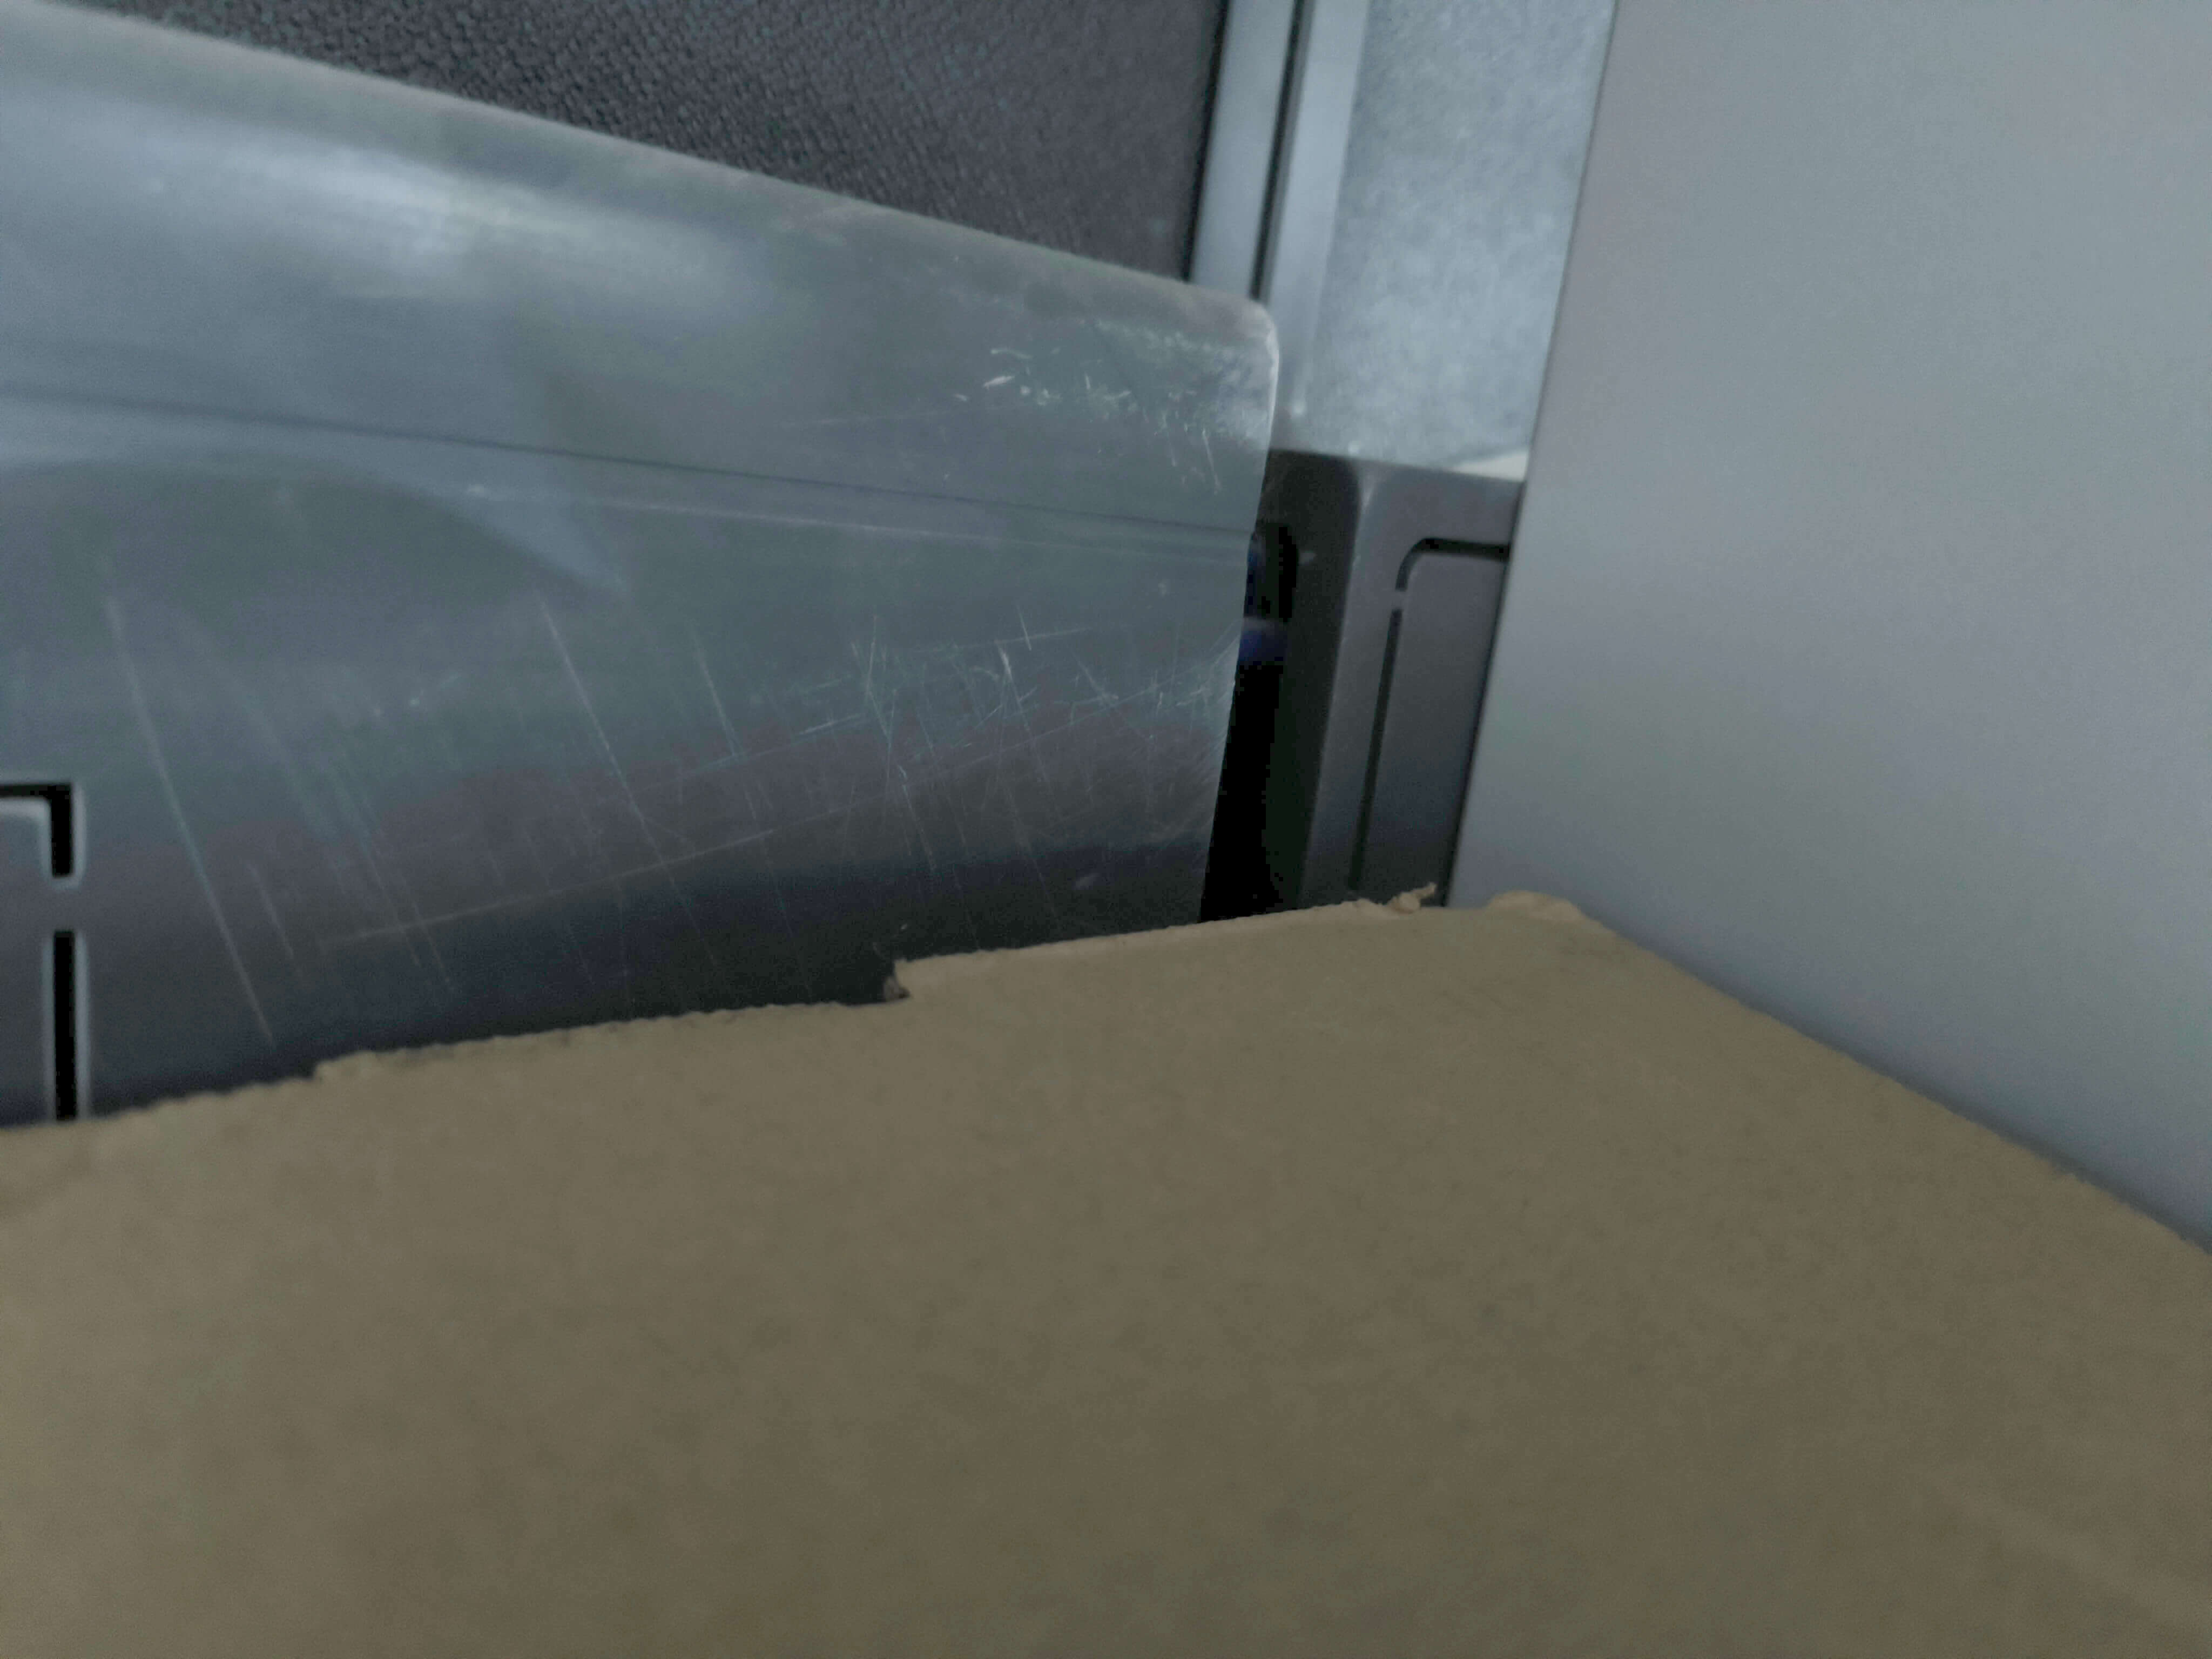
\includegraphics[width=0.32\textwidth]{./coding/2.2.1_results/low_light_levels.jpg}}
  \subfigure[curves]{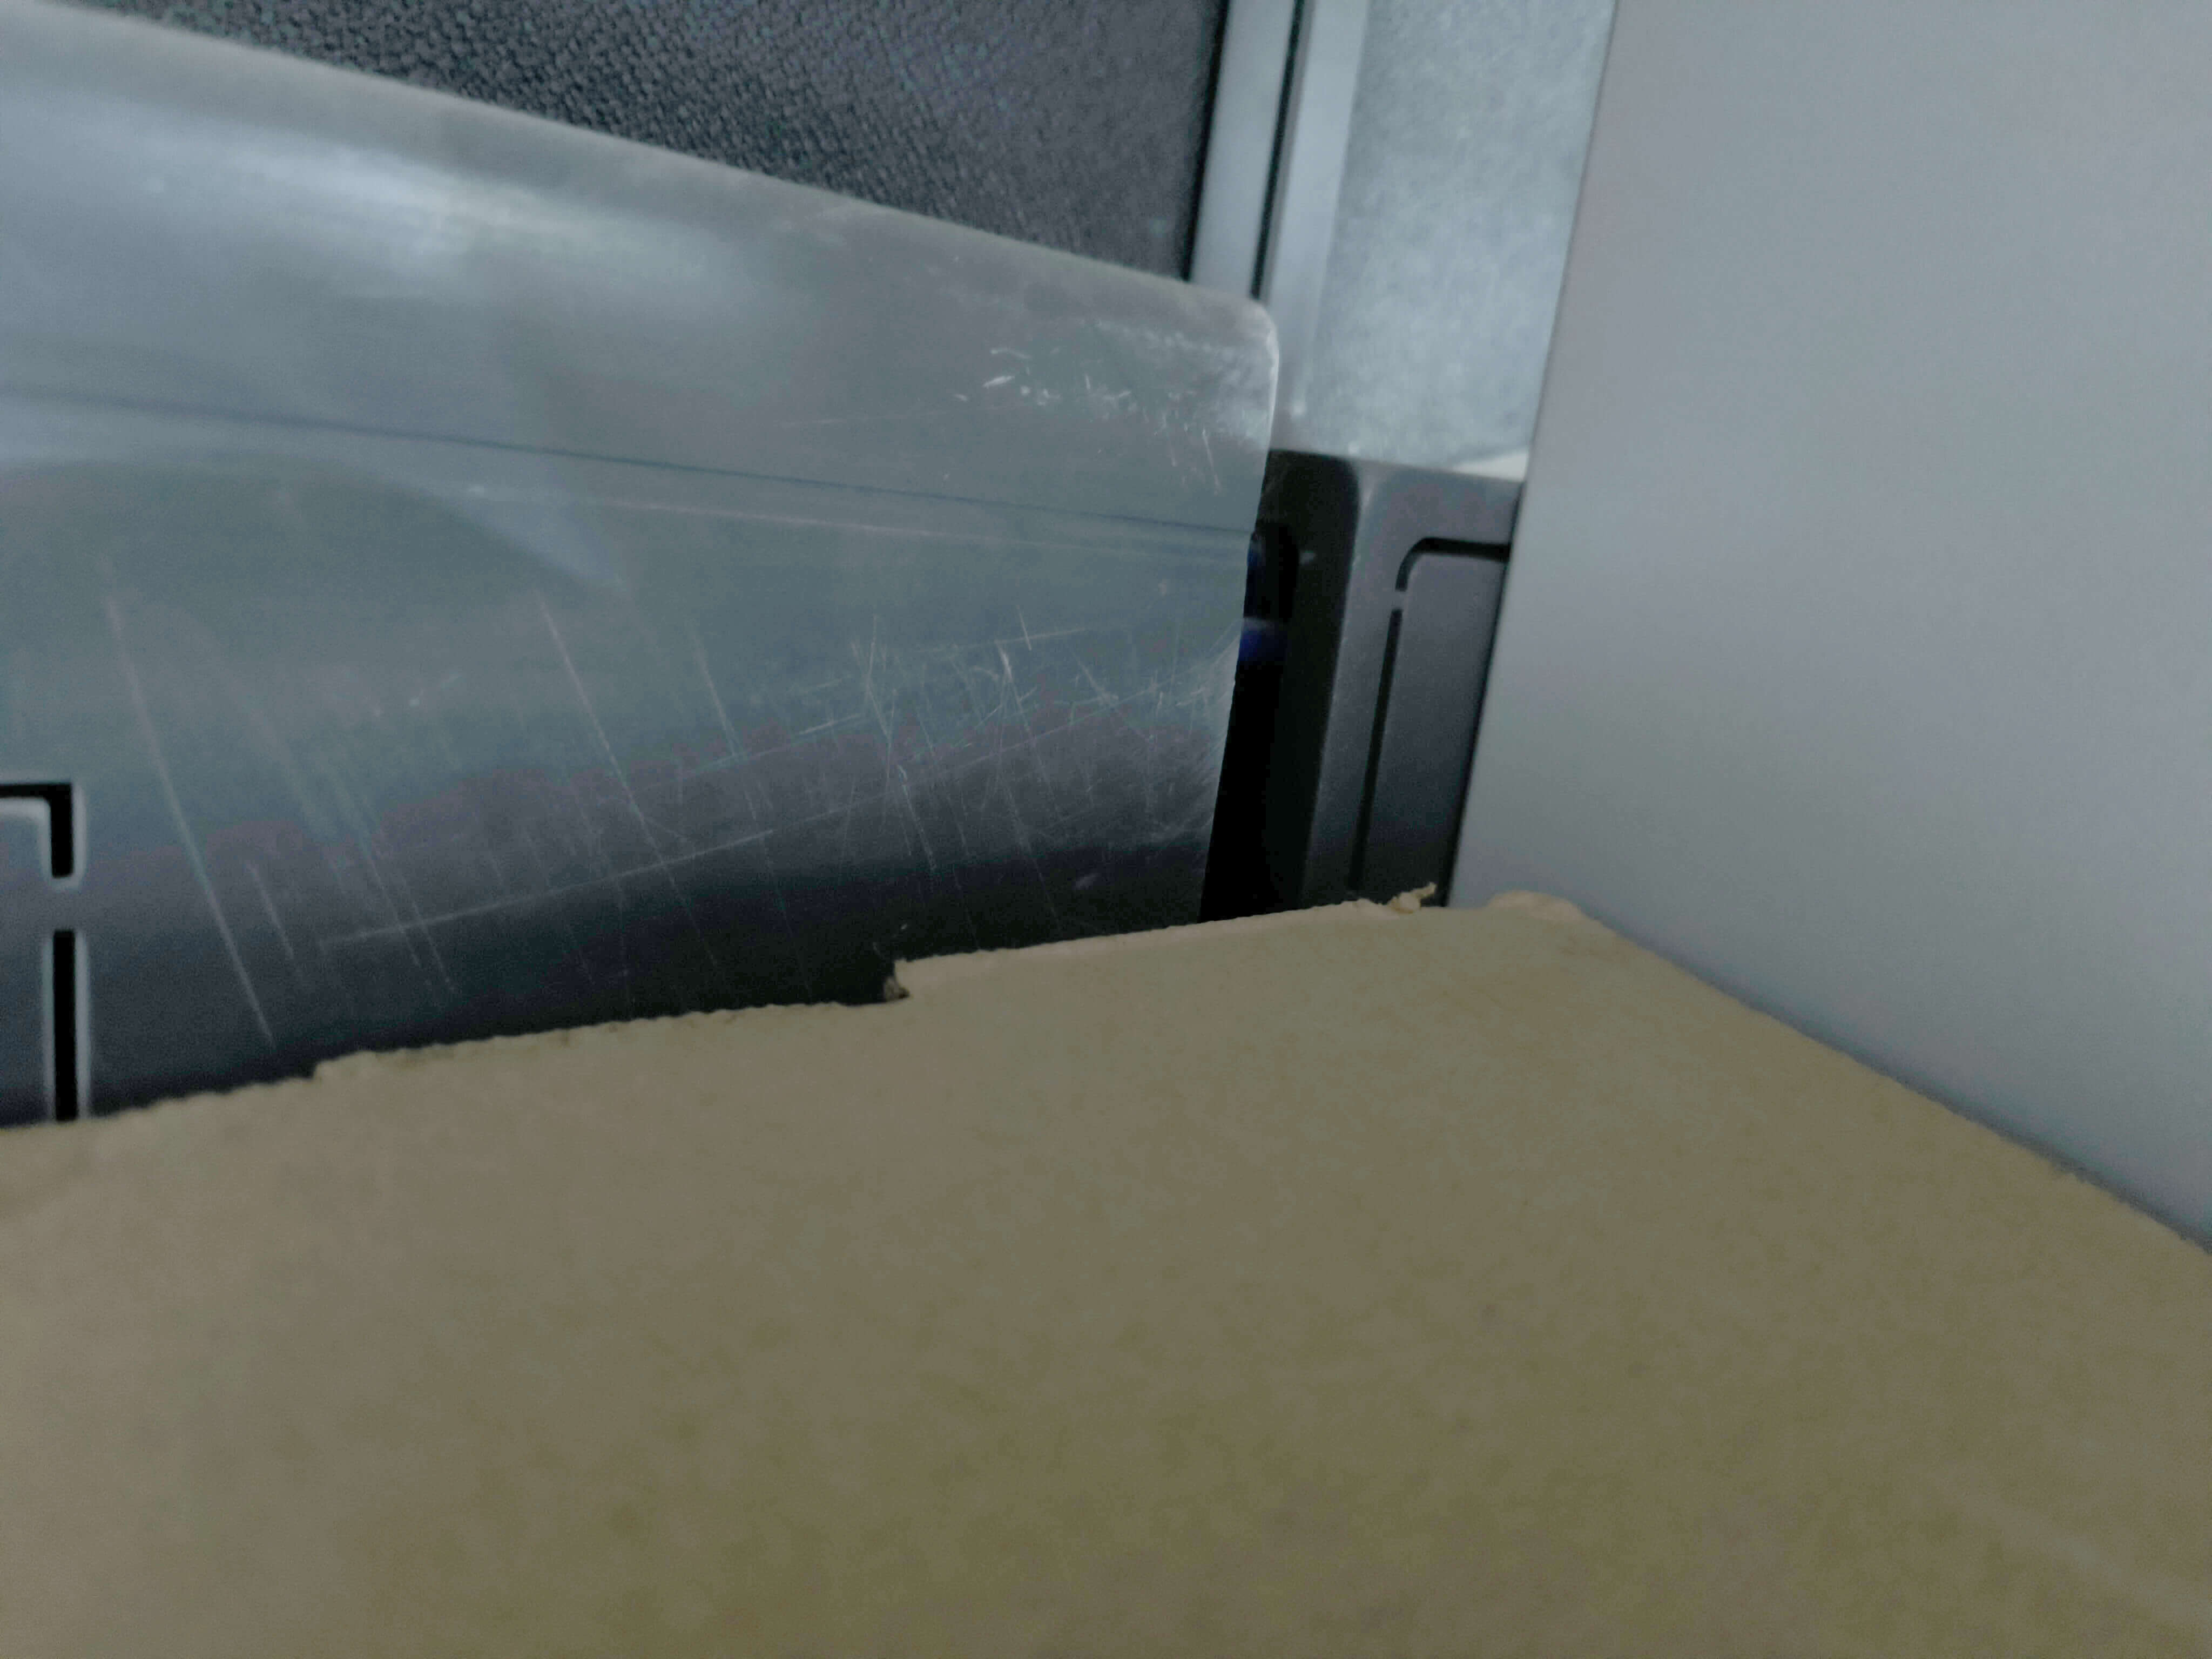
\includegraphics[width=0.32\textwidth]{./coding/2.2.1_results/low_light_curves.jpg}}
  \subfigure[exposure]{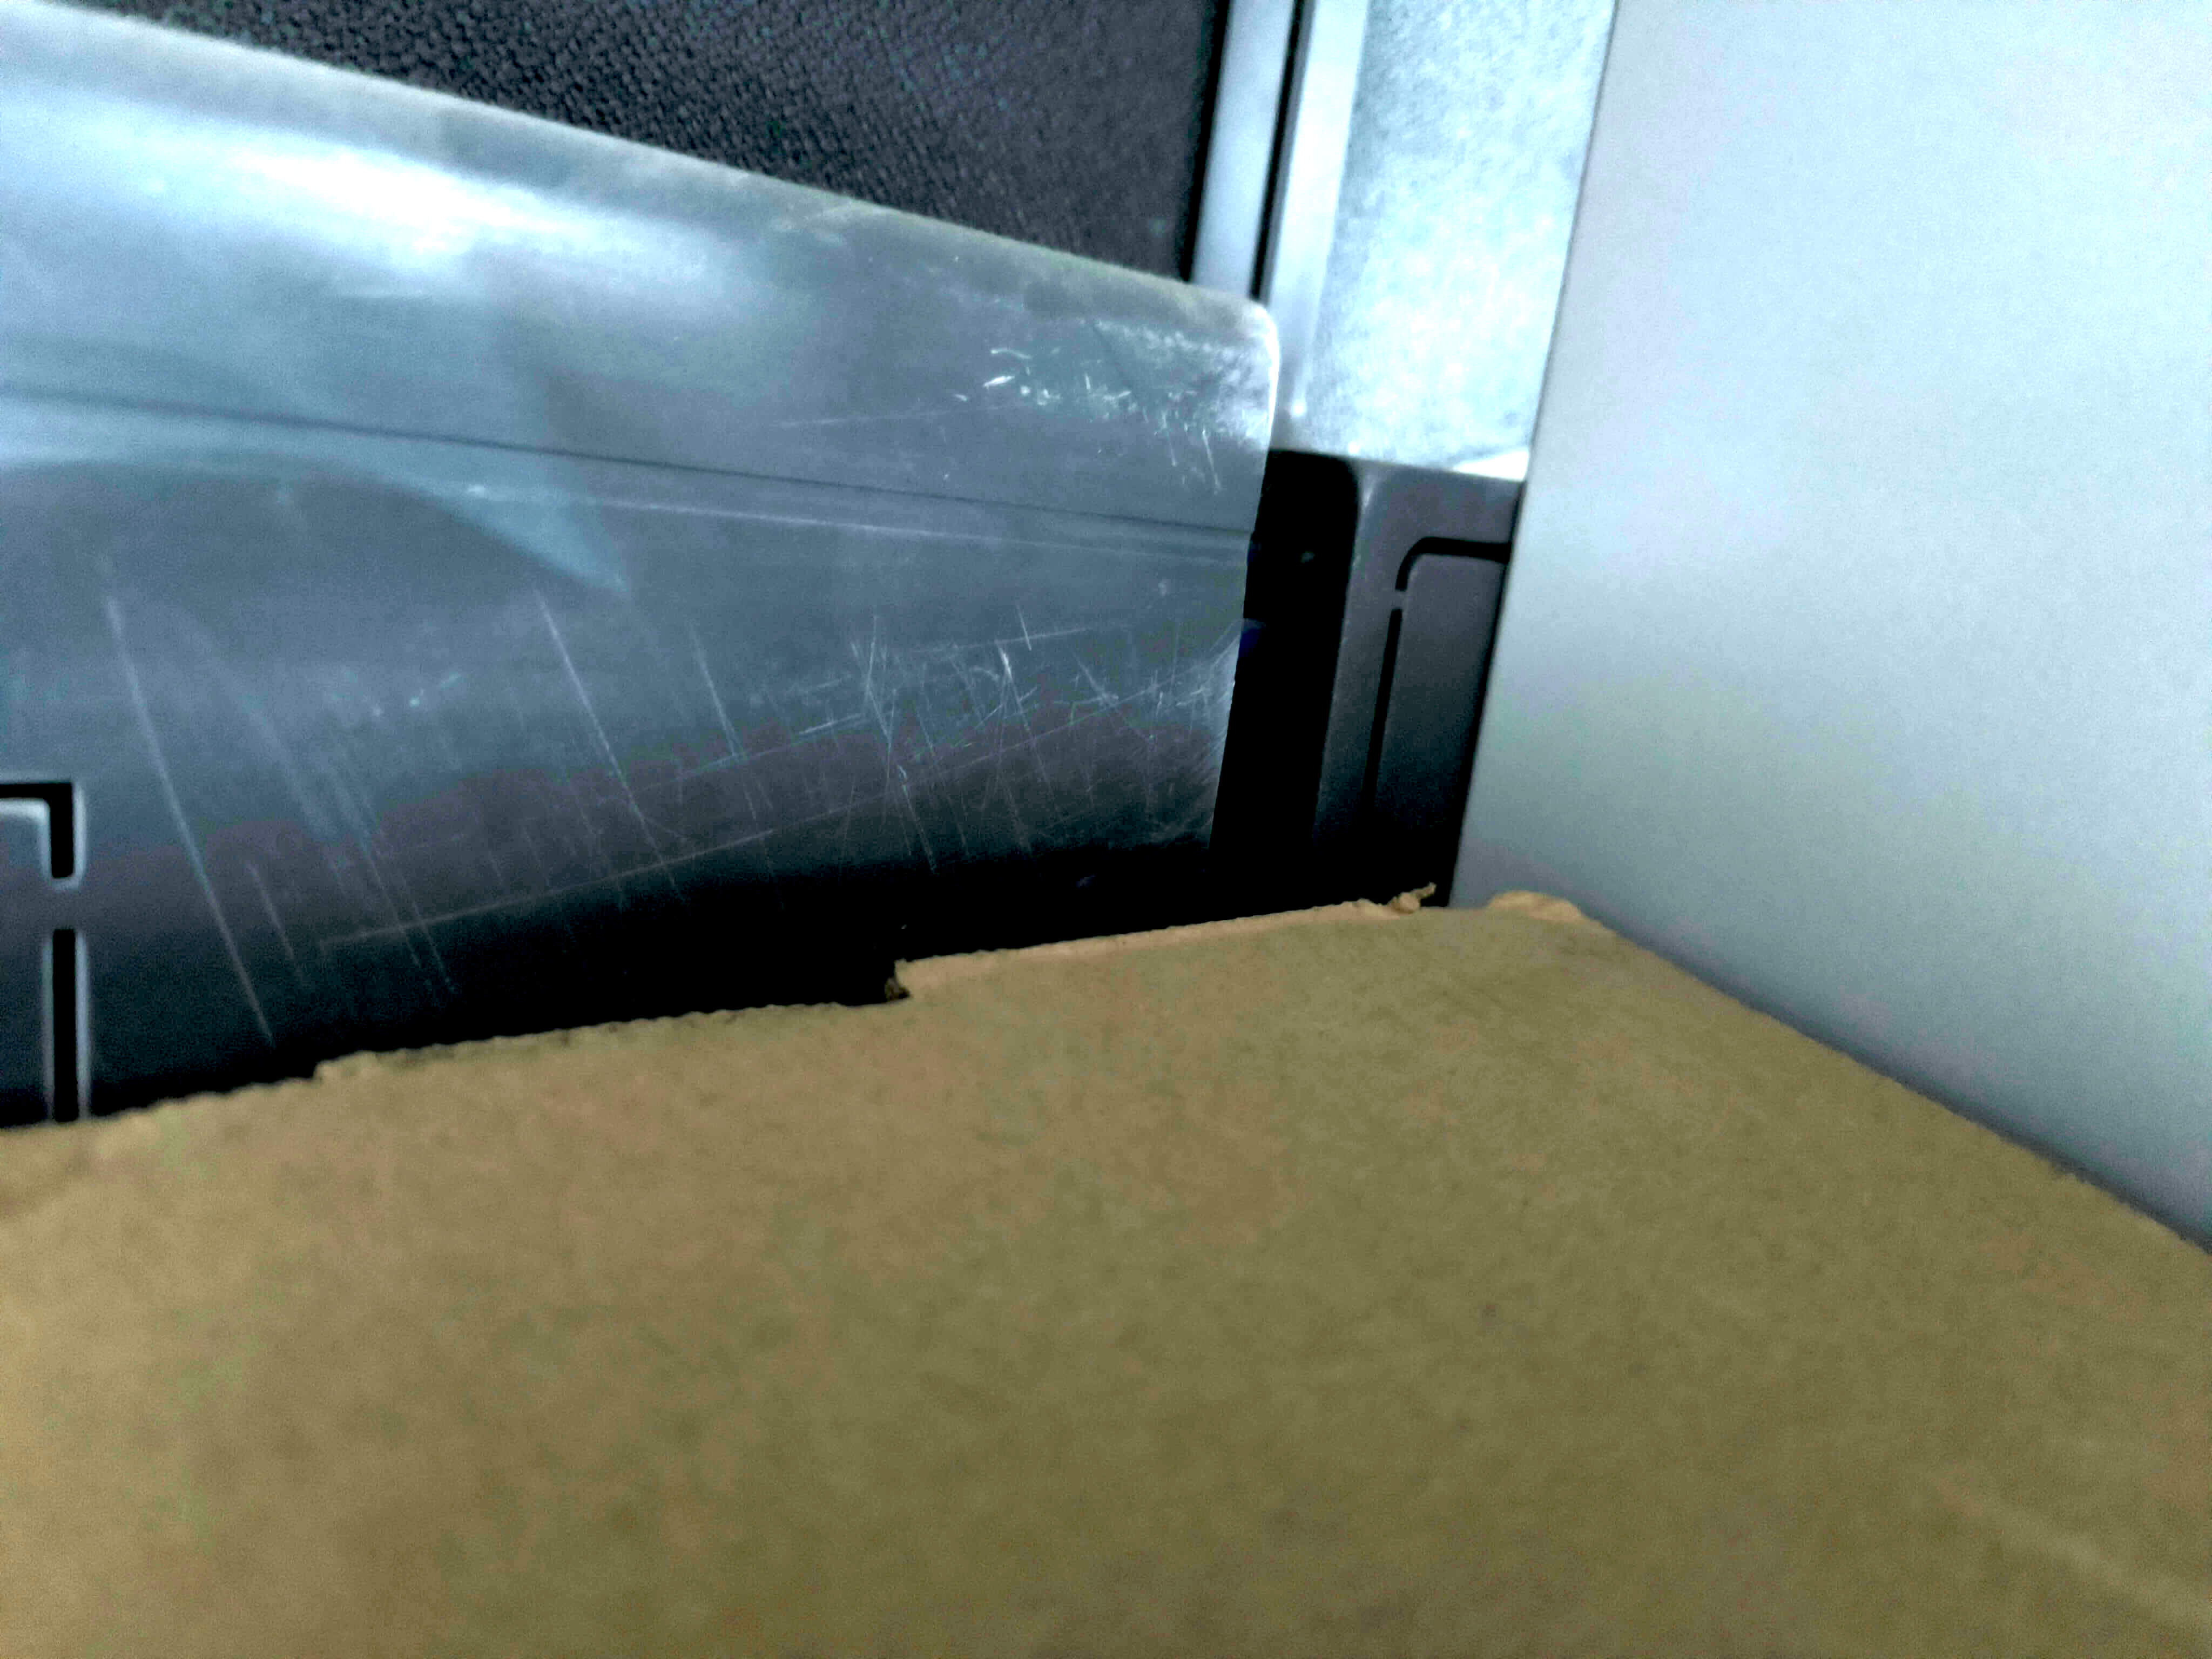
\includegraphics[width=0.32\textwidth]{./coding/2.2.1_results/low_light_exposure.jpg}}
  \setlength{\abovecaptionskip}{0ex}  % 如果使用了minted会增大图像与标题间距需要进行缩小
  \caption{使用PS的四种工具对原图分别进行处理得到的效果图}
\end{figure}
\end{solution}

\begin{problem}
查阅文献,复习和了解Multi-view Geometry (网上有相关的总结材料)。
\end{problem}
\begin{solution}
多视图几何是计算机视觉中的核心内容,旨在从多个图像视角中重建三维场景结构以及相机的运动状态。
\subsubsection*{基本概念}
\begin{itemize}
  \item \textbf{相机模型(Camera Model)}:描述三维点如何投影到二维图像平面。常见模型包括针孔相机模型(Pinhole Model)。
  
  \item \textbf{投影矩阵(Projection Matrix)}:将三维点 $\boldsymbol{X}$ 投影为图像上的二维点 $\boldsymbol{x}$,形式为:
  \[
  \boldsymbol{x} = P X
  \]
  其中,$P = K [R \mid t]$,$K$ 为相机内参矩阵,$R, t$ 分别为旋转矩阵和平移向量。
  
  \item \textbf{基础矩阵(Fundamental Matrix)}:描述两个图像中对应点之间的极几何关系,满足:
  \[
  \boldsymbol{x}'^\top F \boldsymbol{x} = 0
  \]
  
  \item \textbf{本质矩阵(Essential Matrix)}:在归一化相机坐标下的极几何关系,满足:
  \[
  \boldsymbol{x}'^\top E \boldsymbol{x} = 0,\quad E = [t]_\times R
  \]
\end{itemize}

\subsubsection*{典型任务}
\begin{itemize}
  \item \textbf{相机标定(Camera Calibration)}:确定相机的内参矩阵 $K$。
  \item \textbf{特征匹配(Feature Matching)}:识别图像间对应点(如 SIFT, ORB)。
  \item \textbf{三角测量(Triangulation)}:通过两个视角的对应点计算三维点位置。
  \item \textbf{姿态估计(Pose Estimation)}:从2D-3D或2D-2D点对中恢复相机位姿。
  \item \textbf{结构重建(Structure from Motion, SfM)}:从多个图像中联合恢复相机轨迹与三维结构。
\end{itemize}

\subsubsection*{常见方法与工具}
\begin{itemize}
  \item \textbf{8点法(Eight-point Algorithm)}:估计基础矩阵 $F$。
  \item \textbf{PnP 问题(Perspective-n-Point)}:从已知3D点及其图像投影估计相机位姿。
  \item \textbf{束调整(Bundle Adjustment)}:优化相机参数与三维点位置以最小化重投影误差。
\end{itemize}

\subsubsection*{常见参考资料}
\begin{itemize}
  \item R. Hartley and A. Zisserman, \textit{Multiple View Geometry in Computer Vision}, 2nd Edition.
  \item 网上总结资料:\url{https://ksimek.github.io/}
  \item GitHub项目:\url{https://github.com/openMVG/openMVG}
\end{itemize}
\end{solution}

\section{Chapter3}
\subsection{Convolution \& Filtering}
\begin{problem}
学习和实践课件中的不同卷积、线性滤波和非线性滤波的效果。
\end{problem}
\begin{solution}
课件中所提到的卷积、线性滤波和非线性滤波分别有:
\begin{itemize}
  \item 卷积:领域平均滤波,高斯滤波,一阶微分算子、二阶微分算子
  \item 线性滤波:图像的非锐化掩模滤波器$d(x,y) = f(x,y)-(f*g)(x,y)$
  \item 非线性滤波:中值滤波应用与椒盐噪声去除,最大值、最小值滤波
\end{itemize}
\textbf{卷积和线性滤波}处理代码如下:
\mypythonfile{./coding/prob3.1.1\(1\).py}
效果如下:
\begin{figure}[H]
  \centering
  \subfigure[原图]{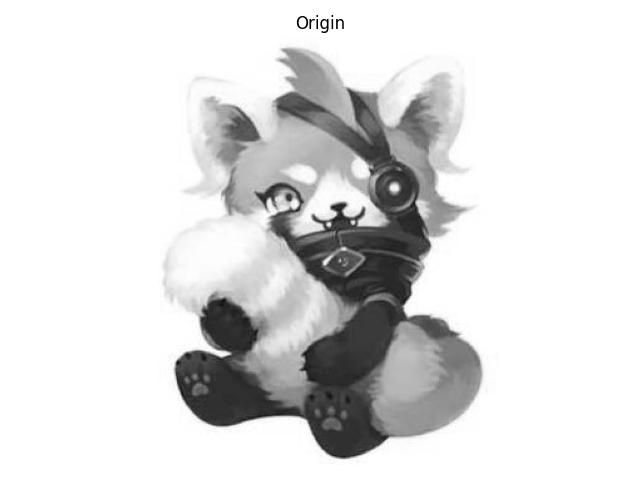
\includegraphics[width=0.32\textwidth]{./coding/3.1.1_results/origin.png}}
  \subfigure[均值滤波, $5\times 5$卷积核]{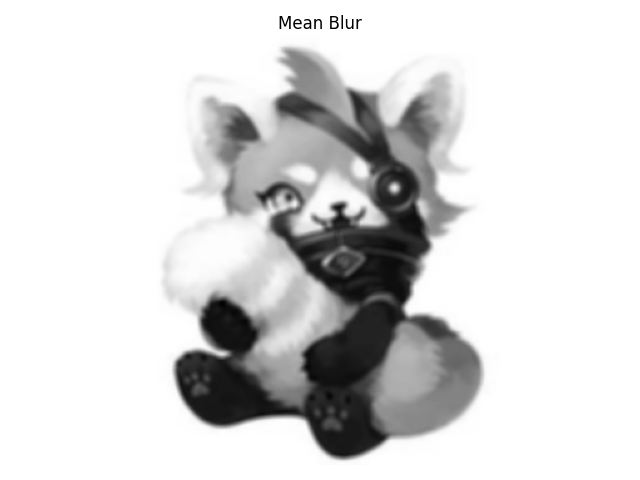
\includegraphics[width=0.32\textwidth]{./coding/3.1.1_results/mean_blur.png}}
  \subfigure[高斯滤波, $5\times 5$卷积核, 方差1]{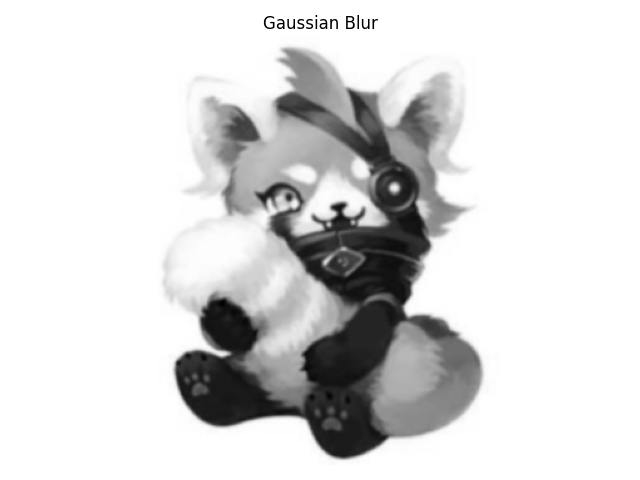
\includegraphics[width=0.32\textwidth]{./coding/3.1.1_results/gaussian_blur.png}}
  \subfigure[一阶微分算子]{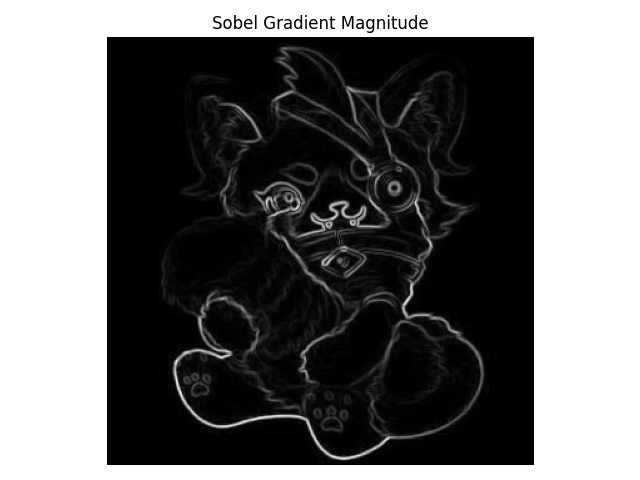
\includegraphics[width=0.32\textwidth]{./coding/3.1.1_results/sobel_gradient_magnitude.png}}
  \subfigure[二阶微分算子]{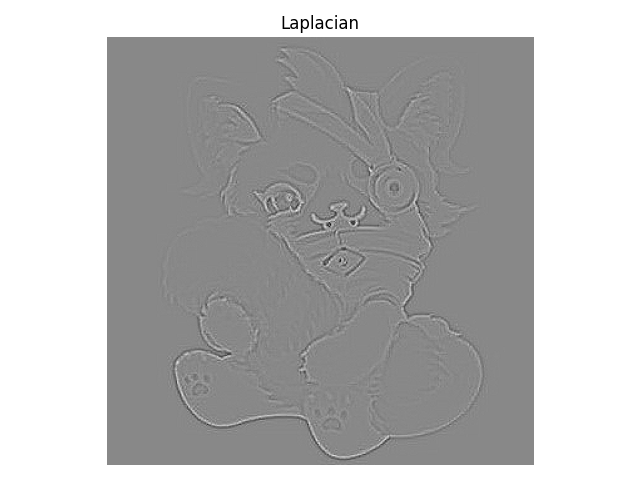
\includegraphics[width=0.32\textwidth]{./coding/3.1.1_results/laplacian.png}}
  \subfigure[非锐化掩模]{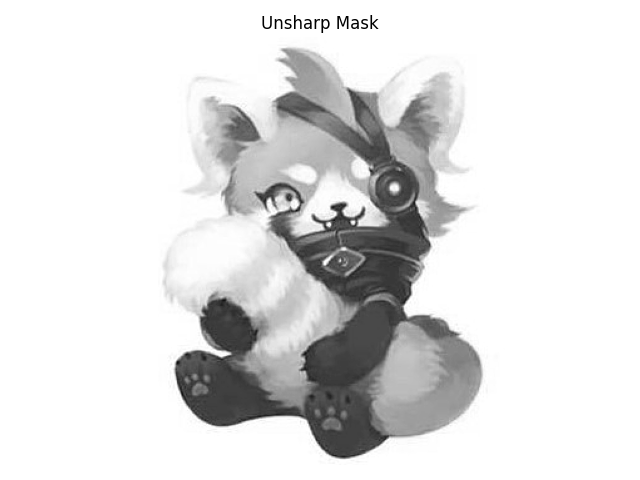
\includegraphics[width=0.32\textwidth]{./coding/3.1.1_results/unsharp_mask.png}}
  \setlength{\abovecaptionskip}{0ex}  % 如果使用了minted会增大图像与标题间距需要进行缩小
  \caption{卷积滤波和线性滤波效果图}
\end{figure}
\clearpage
\textbf{非线性滤波}处理代码如下:
\mypythonfile{./coding/prob3.1.1\(2\).py}
\clearpage
效果如下:
\begin{figure}[H]
  \centering
  \subfigure[原图]{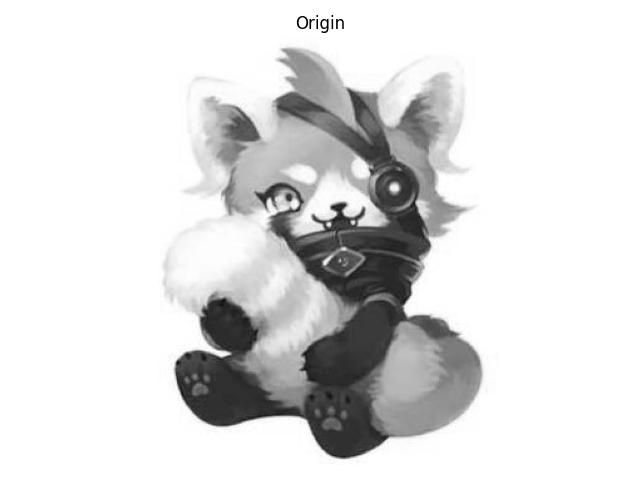
\includegraphics[width=0.32\textwidth]{./coding/3.1.1_results/origin.png}}
  \subfigure[加入椒盐噪声]{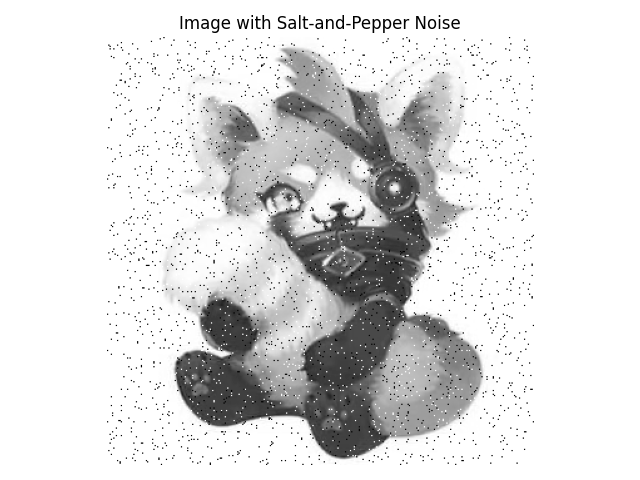
\includegraphics[width=0.32\textwidth]{./coding/3.1.1_results/image_with_salt-and-pepper_noise.png}}
  \subfigure[使用中值滤波去噪]{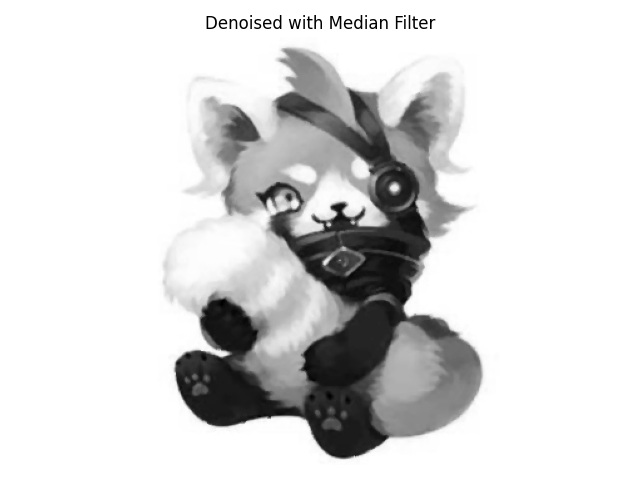
\includegraphics[width=0.32\textwidth]{./coding/3.1.1_results/denoised_with_median_filter.png}}
  \subfigure[使用最大值滤波去噪]{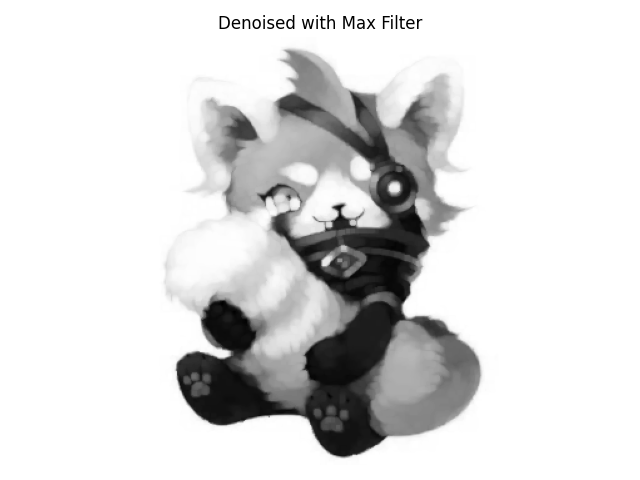
\includegraphics[width=0.32\textwidth]{./coding/3.1.1_results/denoised_with_max_filter.png}}
  \subfigure[使用最小值滤波去噪]{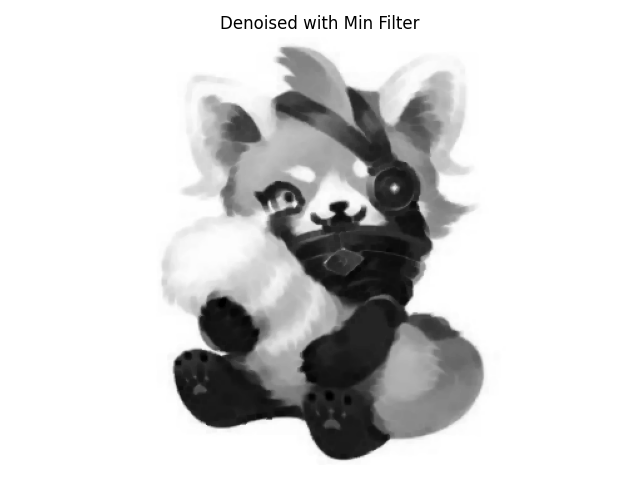
\includegraphics[width=0.32\textwidth]{./coding/3.1.1_results/denoised_with_min_filter.png}}
  \setlength{\abovecaptionskip}{0ex}  % 如果使用了minted会增大图像与标题间距需要进行缩小
  \caption{非线性滤波效果图}
\end{figure}
\end{solution}

\subsection{文本分析的深度学习模型}
\begin{problem}
阅读本次课所讲论文,进一步了解BERT, GPT等大型预训练模型。
\end{problem}
\begin{solution}
\textbf{BERT 与 GPT 等大型预训练语言模型介绍}:近年来,随着计算资源的提升和数据规模的扩展,基于 Transformer 架构的大型预训练语言模型
(Pretrained Language Models, PLMs)已成为自然语言处理的主流技术路线。其中代表性模型包括 BERT、GPT 等。
\subsubsection*{模型结构与基本原理}
BERT 和 GPT 均基于 Transformer 模型,其核心计算过程为多层自注意力机制(self-attention)与前馈神经网络(Feed Forward Network, FFN)的堆叠。Transformer 的输入为一组词嵌入序列 $\boldsymbol{x}_1, \boldsymbol{x}_2, \dots, \boldsymbol{x}_n$,输出为相应位置的上下文表示。

Transformer 的注意力计算形式为:
\[
\text{Attention}(Q, K, V) = \text{softmax} \left( \frac{Q K^\top}{\sqrt{d}} \right) V
\]
其中:
\begin{itemize}
  \item $Q = X W^Q,\quad K = X W^K,\quad V = X W^V$
  \item $X$ 表示输入序列矩阵,$W^Q, W^K, W^V$ 为可学习参数矩阵
\end{itemize}

\subsubsection*{BERT:双向编码器表示模型}
BERT(Bidirectional Encoder Representations from Transformers)使用 Transformer 编码器堆叠,并采用双向注意力机制建模上下文。

\textbf{预训练任务} 包括:
\begin{itemize}
  \item \textbf{掩码语言模型(Masked Language Modeling, MLM)}:
  给定输入 $\boldsymbol{x}_1, \dots, \boldsymbol{x}_n$,随机遮蔽其中部分位置 $\boldsymbol{x}_i$,模型目标为预测被遮蔽的词。
  \item \textbf{下一句预测(Next Sentence Prediction, NSP)}:
  判断两个句子是否在原语料中相邻。
\end{itemize}

BERT 更适用于分类、句对匹配等理解类任务。

\subsubsection*{GPT:自回归生成式模型}

GPT(Generative Pretrained Transformer)使用 Transformer 解码器堆叠,采用单向自注意力结构,适用于语言建模和生成任务。

GPT 的语言建模目标为最大化:

\[
\mathcal{L} = \sum_{t=1}^{n} \log P(\boldsymbol{x}_t \mid \boldsymbol{x}_1, \dots, \boldsymbol{x}_{t-1})
\]

即使用历史上下文预测下一个词。

GPT 更适用于文本生成、对话系统、代码生成等生成类任务。

\subsubsection*{对比与发展趋势}

\begin{itemize}
  \item BERT 使用双向注意力,适合 \textbf{理解类任务}(如问答、文本分类)。
  \item GPT 使用自回归结构,适合 \textbf{生成类任务}(如写作、续写)。
  \item 当前主流发展方向包括:
  \begin{itemize}
    \item 更大规模:如 GPT-3、GPT-4、PaLM、GLM 等;
    \item 多模态融合:如 CLIP、BLIP、GPT-4V 等;
    \item 微调与指令调优:如 InstructGPT、ChatGPT、LLaMA 等;
  \end{itemize}
\end{itemize}

\subsubsection*{参考资料}

\begin{itemize}
  \item BERT 论文:\textit{BERT: Pre-training of Deep Bidirectional Transformers for Language Understanding}
  \item GPT 论文:\textit{Improving Language Understanding by Generative Pre-Training}
  \item Transformer 原始论文:\textit{Attention is All You Need}
  \item 相关开源项目:
  \begin{itemize}
    \item HuggingFace Transformers: \url{https://github.com/huggingface/transformers}
    \item OpenAI API: \url{https://platform.openai.com/}
  \end{itemize}
\end{itemize}

\end{solution}

\section{Chapter 4}
\subsection{Filtering Frequency}
\begin{problem}
基于Python,尝试将图像进行fft变换;在变换域内进行低通、高通滤波等操作,并将滤波后信号用逆fft变换获得图像。
\end{problem}
\begin{solution}
使用\texttt{opencv-python, numpy}即可完成上述fft变换的操作,具体代码如下:
\mypythonfile{./coding/prob4.1.1.py}
效果图如下,左上角为原始图像,中上图为二维fft变换后将低频平移到中心点,
并对范数做$20\log(|x|+1)$变换后的效果图,
右上角为低通滤波频域效果图,
左下角为低通滤波后图像,中下方为高通滤波频域效果图,右下角为高通滤波后的图像(滤波蒙版为半径$30$像素的圆形):
\begin{figure}[htbp]
  \centering
  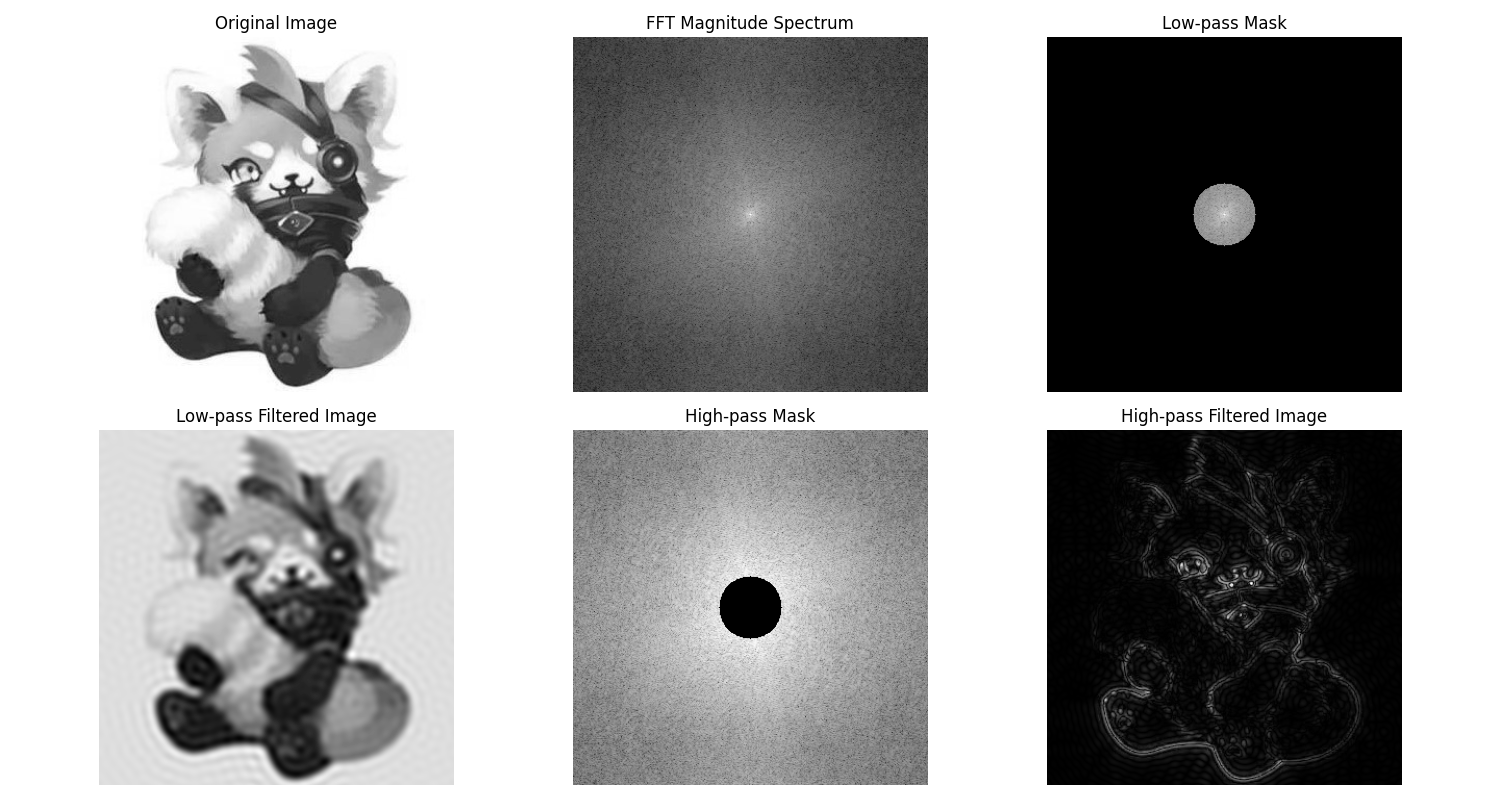
\includegraphics[width=\linewidth]{./coding/4.1.1_results/fft_results.png}
  \caption{fft处理后的效果图}
\end{figure}
\end{solution}
\begin{problem}
课后题4-1:空域有正负值,一旦变为负数不再变为正数,频域/空域的宽窄有什么关系和含义?
\end{problem}
\begin{solution}
当图像在空域中进行某些处理(如锐化、边缘增强、卷积运算)后,像素值可能出现负值。一旦像素值变为负数,若后续处理不具备还原能力,这些值可能持续偏离原始亮度范围,从而导致图像失真甚至信息丢失。

\subsubsection*{频域与空域的宽窄关系}

在图像处理中,空域和频域之间是一对傅里叶变换的对偶关系:

\begin{itemize}
  \item \textbf{空域(Spatial Domain)} 中图像的变化反映了图像的几何结构与局部细节;
  \item \textbf{频域(Frequency Domain)} 中的频率分量描述了图像灰度值变化的快慢:高频对应边缘、细节,低频对应光照、平滑区域。
\end{itemize}

根据傅里叶变换的基本原理,有如下性质:

\begin{center}
  \fbox{
  空域越“窄” $\Rightarrow$ 频域越“宽”;\quad
  空域越“宽” $\Rightarrow$ 频域越“窄”
  }
\end{center}

例如,一个具有尖锐边缘的图像在空域中具有突变(值变化剧烈),对应于频域中的高频成分显著;而一个模糊图像在空域中变化缓慢,其频谱则集中在低频区域。

\subsubsection*{结合问题分析}

当图像处理导致空域中像素变为负值,且此状态在后续处理链条中无法逆转(如未进行适当归一化、截断或修正),说明图像在空域中出现了强烈的局部变化 —— 即突变。

根据频域对偶关系,空域的这种“窄”表现(局部急剧变化)会引起频域谱的扩展,表现为高频成分增强。这种频谱扩展可能导致能量溢出到图像频谱边界,从而产生伪影、边缘噪声等。

\subsubsection*{结论}

\begin{itemize}
  \item 空域中像素值持续为负,反映出图像的剧烈局部变化。
  \item 这种变化在频域中表现为高频能量增加,即频谱变宽。
  \item 空/频域宽窄的本质关系体现了图像表示之间的互补性。
\end{itemize}

因此,在图像设计与滤波操作中,应根据频域响应控制空域行为,避免图像失真或负值扩散现象。
\end{solution}
\section{Chapter 5}
\subsection{文本分析的知识图谱}
\begin{problem}
复习知识图谱的基本概念、基本方法与相关论文。
\end{problem}
\begin{solution}
\subsubsection*{基本概念}
\begin{itemize}
  \item \textbf{信息(Information)}:客观事实的记录,如“水温是7度”。
  \item \textbf{知识(Knowledge)}:对客观规律的总结,如“水在0度时结冰”。
  \item \textbf{知识图谱(Knowledge Graph)}:表示实体之间语义关系的图结构,由三元组组成:
  \[
    (h, r, t) \in \mathcal{E} \times \mathcal{R} \times (\mathcal{E} \cup \mathcal{L})
  \]
  例如:("Microsoft", "based in", "Washington")
\end{itemize}

\subsubsection*{基本方法}
\begin{enumerate}[label=(\arabic*)]
  \item \textbf{逻辑推理(Logical Reasoning)}
  \[
    \text{Parents of Parents} \Rightarrow \text{Grandparents}
  \]
  \item \textbf{知识图谱嵌入(Knowledge Graph Embedding)}:将实体与关系映射到向量空间中进行推理。
  \item \textbf{符号逻辑规则(Symbolic Logical Rules)}:基于Prolog、Markov逻辑网络等方法。
\end{enumerate}

开源工具有
\begin{itemize}
  \item \href{https://github.com/thunlp/OpenKE}{OpenKE}
  \item \href{https://github.com/pykeen/pykeen}{PyKEEN}
  \item \href{https://github.com/facebookresearch/PyTorch-BigGraph}{PyTorch-BigGraph}
  \item \href{https://github.com/awslabs/dgl-ke}{DGL-KE}
  \item \href{https://graphvite.io/}{GraphVite}
\end{itemize}

\subsubsection*{相关论文}
\begin{itemize}
  \item A. Bordes et al., \textit{Translating embeddings for modeling multi-relational data}, NIPS 2013.
  \item T. Trouillon et al., \textit{Complex embeddings for simple link prediction}, ICML 2016.
  \item Z. Sun et al., \textit{RotatE: Knowledge graph embedding by relational rotation in complex space}, ICLR 2019.
  \item M. Schlichtkrull et al., \textit{Modeling relational data with graph convolutional networks}, ESWC 2018.
  \item K. Teru et al., \textit{Inductive relation prediction by subgraph reasoning}, ICML 2020.
\end{itemize}
\end{solution}

\subsection{ImageDegradation \& Restoration}
\begin{problem}
复习双边滤波和非局部滤波方法,尝试上述两种算法做图像去噪。参考程序如下:
\href{http://www.mathworks.com/matlabcentral/fileexchange/13176-non-local-means-filter}{mathworks/non-local-means-filter},
\href{http://www.mathworks.com/matlabcentral/fileexchange/12191-bilateral-filtering}{mathworks/bilateral-filtering}
\end{problem}
\begin{solution}
\subsubsection*{双边滤波}
双边滤波是一种保边缘的图像平滑方法,结合了空间与灰度相似性信息。
设图像为 $I(x)$,双边滤波的输出为:

\[
I^\text{BF}(x) = \frac{1}{W(x)} \sum_{x_i \in \Omega} G_s(\|x - x_i\|) \cdot G_r(|I(x) - I(x_i)|) \cdot I(x_i)
\]
其中:
\begin{itemize}
  \item $G_s$ 是空间距离的高斯函数:$G_s(d) = \exp\left( -\frac{d^2}{2\sigma_s^2} \right)$
  \item $G_r$ 是像素强度差异的高斯函数:$G_r(r) = \exp\left( -\frac{r^2}{2\sigma_r^2} \right)$
  \item $W(x)$ 是归一化因子:
  \[
  W(x) = \sum_{x_i \in \Omega} G_s(\|x - x_i\|) \cdot G_r(|I(x) - I(x_i)|)
  \]
\end{itemize}

\subsubsection*{非局部均值滤波}
非局部均值滤波通过考虑图像中所有具有相似纹理的像素块进行加权平均:

\[
I^\text{NLM}(x) = \frac{1}{C(x)} \sum_{x_i \in \Omega} w(x, x_i) \cdot I(x_i)
\]
其中:
\[
w(x, x_i) = \exp\left( -\frac{\|P(x) - P(x_i)\|^2}{h^2} \right)
\]

\begin{itemize}
  \item $P(x)$ 表示以 $x$ 为中心的图像块
  \item $h$ 是滤波强度控制参数
  \item $C(x)$ 是归一化因子:$C(x) = \sum_{x_i} w(x, x_i)$
\end{itemize}

代码采用\texttt{skimage}包实现,使用\texttt{pip}安装\texttt{pip install scikit-image PyWavelets},代码如下
\pythonfile{./coding/prob5.2.1.py}
效果图如下
\begin{figure}[htbp]
  \centering
  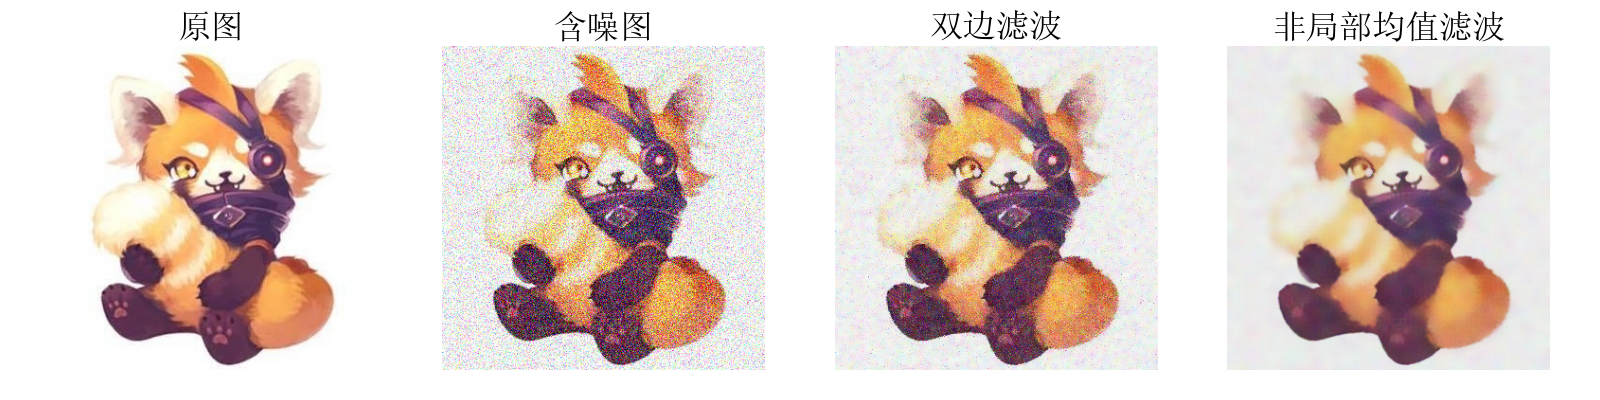
\includegraphics[width=\linewidth]{./coding/5.2.1_results/output.png}
  \caption{双边滤波与非局部均值滤波效果图}
\end{figure}
\end{solution}
\end{document}
